\documentclass[11pt,a4paper]{article}
\usepackage[margin=1in]{geometry}
\usepackage{graphicx}
\usepackage{amsmath}
\usepackage{amssymb}
\usepackage{braket}
\usepackage{color}
\usepackage{url}
\usepackage[numbers,sort&compress]{natbib}
\usepackage{float}
\usepackage{caption}
\usepackage{subcaption}
\usepackage[colorlinks=true,
            linkcolor=blue,
            citecolor=red,
            filecolor=blue,
            menucolor=blue,
            anchorcolor=blue,
            bookmarks=true,
            bookmarksopen=true,
            bookmarksnumbered=true,
            pdfstartview=FitH,
            pdftitle={A Generalized PyTheus Quantum Network Interpreter},
            pdfauthor={S. K. Rithvik},
            pdfsubject={Quantum Network Analysis},
            pdfkeywords={quantum networks, PyTheus, automated design, network interpretation}]{hyperref}

% Title formatting
\usepackage{titling}
\setlength{\droptitle}{-2em}

% Custom commands for author and affiliation formatting
\usepackage{authblk}
\renewcommand\Authfont{\normalsize\bfseries}
\renewcommand\Affilfont{\small\itshape}
\setlength{\affilsep}{0.5em}

\begin{document}

\title{A Modular PyTheus Quantum Network Interpreter:\\
Automated Analysis and Visualization of Optimized Quantum Architectures}

\author[1,2]{S. K. Rithvik\thanks{Corresponding author. Email: rithvik\_ks@iitgn.ac.in}}
\affil[1]{Quantum Science and Technology Laboratory, Physical Research Laboratory, Navrangpura, Ahmedabad 380009, India}
\affil[2]{Indian Institute of Technology Gandhinagar, Palaj, Gandhinagar 382355, India}

\date{\today}

\maketitle

\begin{abstract}
We present a modular interpreter for PyTheus-optimized quantum networks that automatically analyzes and visualizes complex quantum architectures discovered through automated optimization. The interpreter addresses the critical challenge of understanding machine-designed quantum networks by providing robust algorithms for functional role identification, graph-theoretical analysis, and physically meaningful visualization across the major classes of PyTheus-generated networks. Our interpreter accepts both file-based and in-memory network representations, automatically identifies sources, detectors, beam splitters, and ancillas through priority-based classification, and generates coordinated native graph plots and optical table representations. We demonstrate the interpreter's capabilities through two complementary approaches: (1) analysis of a newly developed five-node quantum key distribution network that reveals distributed source architecture and dual-role node functionality, and (2) comprehensive validation using existing PyTheus examples including W4 state generation, heralded Bell state preparation, and GHZ state networks. The interpreter successfully handles complex connectivity patterns across diverse quantum network architectures within the tested classes, avoids visualization artifacts, and provides validation mechanisms for architectural consistency. Our primary contribution is the development of robust modular interpretation algorithms that can analyze the major classes of PyTheus-generated quantum networks, enabling better understanding of automated quantum architecture design.
\end{abstract}

\section{Introduction}

The automated design of quantum networks has emerged as a critical capability for developing large-scale quantum communication and computing systems. Tools like the PyTheus quantum optimization framework~\cite{pytheus_reference} can discover complex network architectures that maximize performance objectives, often identifying non-intuitive designs that outperform human-designed alternatives. However, a significant challenge in automated quantum network design is the interpretation and validation of machine-generated architectures.

PyTheus and similar optimization frameworks typically output abstract graph representations with numerical edge weights and vertex configurations. While these representations fully specify the quantum network, they can be difficult for researchers to understand, validate, and translate into physical implementations. The complexity of interpreting these outputs increases dramatically with network size and the sophistication of discovered architectures.

This interpretation challenge has several important consequences: (1) researchers may miss key insights about discovered architectures, (2) validation of optimization results becomes difficult without manual analysis, (3) translation to experimental implementations requires extensive expert interpretation, and (4) comparison between different optimized designs lacks systematic approaches.

In this work, we address these challenges by developing a modular interpreter for PyTheus quantum network outputs. Our interpreter provides automated analysis capabilities that extract meaningful architectural insights from raw optimization results for the major classes of quantum networks produced by PyTheus. The interpreter is designed to handle network configurations within the tested classes and demonstrates robust scalability to networks of varying size and complexity within these domains.

The primary contributions of this work are:
\begin{enumerate}
\item A robust interpreter architecture for analyzing PyTheus quantum network outputs
\item Automated algorithms for functional role identification (sources, detectors, beam splitters, ancillas)
\item Coordinated visualization capabilities producing both graph-theoretical and optical table representations
\item Validation mechanisms ensuring architectural consistency and identifying potential issues
\item Demonstration of interpreter capabilities through new network development (five-node QKD) and comprehensive validation using existing PyTheus examples (W4 state generation, heralded Bell state preparation, and GHZ state networks)
\end{enumerate}

\section{PyTheus Network Interpreter Architecture}

\subsection{Core Design Philosophy}

Our PyTheus interpreter represents a flexible, extensible framework for quantum network analysis that adapts to different network architectures through configurable analysis pipelines. The interpreter employs a multi-priority approach that combines explicit configuration specifications with structural graph analysis to identify functional roles and generate appropriate visualizations.

The interpreter's core philosophy centers on three principles: (1) \textbf{Adaptive Framework} -- a flexible template that can be extended for new quantum network types while providing robust analysis for known architectures; (2) \textbf{Multi-Priority Analysis} -- functional roles are determined through a hierarchy that prioritizes configuration data (such as \texttt{single\_emitters}, \texttt{out\_nodes}, \texttt{anc\_detectors}) over structural heuristics, ensuring reliable analysis across different network types; and (3) \textbf{Coordinated Visualization} -- mathematical graph representations and physical optical layouts maintain strict consistency through synchronized analysis pipelines.

The framework demonstrates strong generality for the PyTheus network types encountered in quantum optics research (W states, Bell states, GHZ states, QKD networks), while maintaining extensibility for new architectures through its modular design and configurable analysis methods.

\subsection{Multi-Modal Input Processing}

The interpreter provides flexible input handling through the \texttt{General\-Quantum\-Network\-\\Interpreter} class constructor, which accepts both file-based and in-memory data structures. The system supports three input modes: (1) file paths to JSON configuration and graph files, (2) direct Python dictionary data via \texttt{config\_data} and \texttt{graph\_data} parameters, and (3) mixed input modes combining file and dictionary inputs. This flexibility enables seamless integration into automated PyTheus optimization workflows while supporting interactive analysis sessions.

The input processing pipeline includes robust error handling and format detection through the \texttt{load\_config} and \texttt{load\_graph} methods. The \texttt{load\_graph\_data} method handles different graph formats by detecting whether graph data is nested under a 'graph' key or provided directly. The \texttt{\_extract\_vertices} method parses PyTheus edge tuples in the format \texttt{(v1, v2, mode1, mode2)} to extract vertex sets, while also supporting simplified \texttt{(v1, v2)} edge formats for basic connectivity analysis.

\subsection{Adaptive Structural Analysis}

The interpreter's structural analysis pipeline operates through the \texttt{analyze\_network\_structure} method, which orchestrates five integrated analysis modules:

\textbf{Graph Topology Analysis}: The \texttt{\_compute\_vertex\_degrees} method calculates vertex degrees from edge data, while \texttt{\_analyze\_connectivity} employs NetworkX algorithms to compute network properties including connectivity components, diameter, average clustering coefficient, and graph density. The system identifies structural patterns through NetworkX's \texttt{is\_tree}, \texttt{is\_bipartite}, and connectivity analysis methods.

\textbf{Functional Role Identification}: The \texttt{\_identify\_functional\_roles} method implements a hierarchical priority system that systematically combines configuration data with structural analysis. The algorithm implements a three-tier priority cascade: (1) explicit configuration specifications take precedence (such as \texttt{single\_emitters}, \texttt{out\_nodes}, \texttt{anc\_detectors}); (2) target state analysis provides secondary guidance through state string length analysis for networks without explicit role specifications; (3) structural heuristics including degree analysis, centrality measures, and connectivity patterns serve as fallback identification methods. The system supports this through four specialized methods: 
\begin{itemize}
\item \texttt{\_identify\_actual\_sources}
\item \texttt{\_identify\_actual\_detectors}
\item \texttt{\_identify\_beam\_splitter\_nodes}
\item \texttt{\_identify\_ancilla\_nodes}
\end{itemize}

\textbf{Mode Analysis}: The \texttt{\_analyze\_modes} method examines optical mode patterns extracted from PyTheus edge tuples, identifying unique mode indices, mode pairing patterns, and coupling strength distributions. The system analyzes edge weight patterns to detect perfect correlations (±1.0) and intermediate coupling strengths, while tracking complex weight distributions for quantum interference analysis.

\textbf{Implementation Strategy Determination}: The \texttt{\_determine\_implementation\_\\strategy} method integrates outputs from all previous analysis modules to determine optical implementation requirements. The system classifies network components through the specialized identification methods and assesses implementation complexity using the \texttt{\_assess\_complexity} method, which considers vertex count, mode complexity, and ancilla requirements to assign complexity levels (simple, moderate, complex).

\textbf{Quantum State Analysis}: The \texttt{\_analyze\_quantum\_state} method processes target state specifications from the configuration, analyzing basis state structures, photon number distributions, and entanglement patterns. The system includes \texttt{\_classify\_entanglement\_type} functionality that recognizes common quantum state patterns (W states, GHZ states, Bell states) based on target state structure.

\subsection{Visualization Generation Pipeline}

The interpreter implements a coordinated dual-visualization approach through two primary methods that generate both native graph plots and optical table representations from the same underlying network analysis.

\textbf{Native Graph Visualization}: The \texttt{plot\_native\_graph} method recreates PyTheus's visual style through circular vertex positioning using \texttt{nx.circular\_layout}, PyTheus-compatible edge coloring where mode indices map to specific colors (dodgerblue for mode 0, firebrick for mode 1, limegreen for mode 2), and adaptive edge thickness scaling based on coupling strength magnitudes. The visualization preserves PyTheus's vertex numbering and layout conventions while providing clear visual representation of network connectivity and coupling patterns.

\textbf{Optical Table Generation}: The \texttt{plot\_optical\_table\_\\setup} method implements a strategy-based approach that automatically selects appropriate plotting methods based on network configuration analysis. The system employs a three-strategy decision tree:
\begin{enumerate}
\item Networks with \texttt{single\_emitters} configuration trigger \texttt{\_plot\_single\_photon\_\\optical\_table} for single-photon source networks (W4, etc.)
\item Networks with both \texttt{out\_nodes} and \texttt{anc\_detectors} configurations trigger \texttt{\_plot\_general\_spdc\_\\optical\_table} for multi-party QKD networks with ancilla heralding
\item All other networks use \texttt{\_plot\_adaptive\_quantum\_\\network} for general quantum network topologies
\end{enumerate}

Each plotting strategy implements specialized optical element positioning:
\begin{itemize}
\item \texttt{\_plot\_single\_photon\_optical\_\\table} renders diamond-shaped single-photon sources with 810nm wavelength specifications
\item \texttt{\_plot\_general\_spdc\_optical\_\\table} implements SPDC architectures with pump lasers (405nm), BBO crystals, and signal/idler outputs
\item \texttt{\_plot\_adaptive\_quantum\_\\network} provides flexible component positioning for diverse network types
\end{itemize} The system implements optical routing through \texttt{\_draw\_optical\_routing} and \texttt{\_draw\_adaptive\_optical\_\\routing} methods that follow physically realistic optical paths while maintaining PyTheus color scheme consistency for multi-mode visualization.

\subsection{Framework Extensibility and Limitations}

The interpreter framework demonstrates strong extensibility through its modular design and configurable analysis pipelines. New quantum network types can be accommodated through several mechanisms: (1) extension of the priority cascade in functional role identification to recognize new configuration patterns, (2) addition of new plotting strategies to the visualization pipeline for network types requiring specialized optical implementations, and (3) modification of the structural analysis methods to recognize novel graph motifs and connectivity patterns.

However, the framework's generality has practical boundaries. The current implementation is optimized for photonic quantum networks with discrete vertex-edge structures typical of PyTheus outputs. Networks with continuous variables, non-photonic implementations, or fundamentally different mathematical representations may require substantial modifications to the analysis pipeline. The optical table visualization strategies, while adaptable, assume standard optical elements (sources, beam splitters, detectors) and may need extension for exotic optical implementations.

The interpreter's strength lies in its demonstrated ability to handle the diverse network types encountered in quantum optics research while maintaining a consistent, extensible architecture that can evolve with new requirements. The multi-priority analysis approach provides a robust foundation for accommodating new network specifications while preserving compatibility with existing configurations.

\subsection{Validation and Consistency Mechanisms}

The interpreter incorporates multiple validation layers to ensure analysis reliability and visualization accuracy. The \texttt{\_analyze\_connectivity} method employs NetworkX algorithms to validate graph consistency through connectivity analysis, computing essential network properties (diameter, clustering coefficient, density) and identifying disconnected components or structural anomalies. The system validates edge weight distributions to ensure coupling strengths remain within physically meaningful ranges and identifies potential issues with perfect correlations (±1.0) versus intermediate coupling values.

The visualization pipeline includes consistency verification through the optical table generation process, which validates that all identified network components have appropriate optical connectivity paths. The multi-priority role identification system incorporates cross-validation between configuration specifications and structural analysis, flagging potential inconsistencies where configuration data conflicts with graph topology. The system performs basic photon number conservation checks by validating that identified source capabilities can generate the photon numbers required by target states, though this validation assumes standard optical implementations and may require extension for exotic quantum architectures.

The \texttt{run\_complete\_analysis} method includes output validation to ensure all generated files maintain consistency in component labeling, color schemes, and technical specifications across optical table plots, native graphs, and text reports.

\subsection{API Design and Integration}

The interpreter provides a clean object-oriented interface through the \texttt{Modular\-Quantum\-Network\-Interpreter} class, which supports flexible instantiation with file paths, dictionary data, or mixed input modes. The primary analysis interface centers on the \texttt{analyze\_network\_structure} method, which returns a comprehensive dictionary containing all network analysis results including vertex properties, functional roles, implementation strategies, and quantum state analysis.

The system implements specialized analysis methods accessible through the main interface: \texttt{\_compute\_vertex\_degrees} for basic graph topology analysis, \texttt{\_analyze\_connectivity} for advanced NetworkX-based graph metrics (clustering, diameter, density), and \texttt{\_find\_graph\_motifs} for structural pattern detection. The role identification system provides direct access to component classification through specialized methods:
\begin{itemize}
\item \texttt{\_identify\_actual\_sources}
\item \texttt{\_identify\_actual\_detectors}
\item \texttt{\_identify\_beam\_splitter\_nodes}
\item \texttt{\_identify\_ancilla\_nodes}
\end{itemize}

The \texttt{run\_complete\_analysis} method provides a streamlined interface for generating all output formats simultaneously. This method executes the complete analysis pipeline and produces three coordinated outputs: optical table plots (via \texttt{plot\_optical\_table\_setup}), native graph visualizations (via \texttt{plot\_native\_graph}), and comprehensive text reports (via \texttt{generate\_analysis\_\\report}). All outputs maintain consistent filename prefixes and include embedded metadata for traceability and reproducibility.

\section{Demonstration and Validation Methodology}

\subsection{Dual-Track Validation Approach}

To comprehensively demonstrate the interpreter's capabilities and validate its generality, we employ a dual-track approach that combines new network development with systematic validation using existing PyTheus examples.

\textbf{Track 1: New Network Development} -- We develop and analyze a sophisticated five-node quantum key distribution (QKD) network that represents a novel architecture optimized for maximum entanglement distribution and secure communication. This network showcases the interpreter's ability to handle complex, previously unseen architectures and reveals design principles that would be difficult to identify through manual analysis.

\textbf{Track 2: Systematic Validation Using Existing Examples} -- We validate the interpreter's generality by applying it to well-established PyTheus examples including:
\begin{itemize}
\item \textbf{W4 State Generation}: A 4-party W state network demonstrating symmetric multiparty entanglement
\item \textbf{Heralded Bell State Preparation}: A sophisticated 2-party Bell state network with heralding mechanisms
\item \textbf{GHZ State Networks}: Multi-party GHZ state generation showcasing central hub architectures
\end{itemize}

This dual-track approach ensures that our interpreter can handle both novel architectures (demonstrating research value) and established configurations (validating correctness and generality).

\subsection{Validation Metrics and Success Criteria}

Our validation methodology employs multiple criteria to assess interpreter performance:

\textbf{Structural Consistency}: The interpreter must correctly identify functional roles (sources, detectors, beam splitters, ancillas) across all network types without manual parameter adjustment.

\textbf{Visualization Quality}: Generated native graph plots and optical table representations must be physically meaningful, uncluttered, and consistent with quantum network theory.

\textbf{Cross-Network Robustness}: The interpreter must handle diverse topologies, from hub-and-spoke architectures to distributed networks, without degradation in analysis quality.

\textbf{Self-Consistency Validation}: All interpreter outputs are validated for internal consistency between graph structure, functional role assignments, and optical table representations to ensure architectural coherence.

\section{New Network Development: Five-Node QKD Case Study}

\subsection{Network Architecture and Optimization Context}

The five-node quantum key distribution (QKD) network represents a sophisticated architecture optimized through PyTheus for secure multi-party communication. Unlike traditional point-to-point QKD protocols, this network enables simultaneous secure communication between five parties through a carefully designed quantum architecture that maximizes entanglement distribution while minimizing operational losses.

The network emerged from an optimization process targeting maximum entanglement distribution across all communication parties. PyTheus employed the L-BFGS-B optimization algorithm with a concurrence-based loss function, exploring 35 potential edge configurations while maintaining 25 samples per iteration, ultimately discovering a 31-edge architecture that satisfies all physical constraints while maximizing the target performance metrics.

The optimization process identified a network topology that challenges conventional assumptions about quantum communication architectures. Rather than employing symmetric hub-and-spoke or fully connected designs, the discovered architecture exhibits strategic asymmetries that optimize performance for the specific five-party communication requirements.

\subsection{Quantum State Structure and Physical Implementation}

The target quantum state for the five-node QKD network consists of a carefully balanced superposition of ten computational basis states, each containing exactly two photons:

\begin{align}
\ket{\psi_{\text{QKD}}} &= \frac{1}{\sqrt{10}} \big( \ket{00011} + \ket{00101} + \ket{01001} + \ket{10001} + \ket{01010} \nonumber \\
&\quad + \ket{10010} + \ket{10100} + \ket{11000} + \ket{00110} + \ket{01100} \big)
\end{align}

This state structure embodies several remarkable physical properties that make it ideal for multi-party QKD applications. The exact two-photon structure enables implementation using spontaneous parametric down-conversion (SPDC) sources, providing reliable photon pair generation with well-controlled spectral and temporal properties. Each communication party (corresponding to the first five qubit positions) appears in exactly four of the ten basis states, ensuring symmetric participation in the quantum communication protocol.

The balanced pairwise correlations inherent in this state structure prevent any bipartite subset from dominating the entanglement distribution, crucial for maintaining security across all communication links. The ten-state superposition provides sufficient quantum advantage for secure key generation while remaining implementable with current optical quantum technology.

\subsection{Network Topology and Connectivity Analysis}

The PyTheus optimization discovered a 10-vertex, 31-edge network architecture that exhibits sophisticated connectivity patterns. The network demonstrates high density (0.6222) indicating substantial interconnection between nodes, with a moderate clustering coefficient (0.4905) revealing significant local structure and tightly connected subnetworks. The compact diameter of 2 ensures efficient information flow, with no node requiring more than two hops to reach any other node.

The network topology analysis reveals rich structural complexity with 24 triangle motifs and 89 square motifs, indicating robust local connectivity patterns that support quantum correlations. Node 3 emerges as the primary hub with the highest degree (9 connections), while the network maintains a balanced degree distribution with nodes ranging from 4 to 9 connections (mean degree 6.2, standard deviation 1.4).

The architecture demonstrates strategic asymmetry optimized for the five-party communication requirements. Communication nodes (0-4) serve as output nodes with degrees ranging from 4 to 9, while ancilla detectors (5-9) function as beam splitters with degrees from 4 to 7, creating a carefully balanced load distribution across the optical infrastructure. The complete network structure is shown in Figure~\ref{fig:5node_qkd_analysis}.

\subsection{Functional Role Identification and Network Architecture}

The interpreter's analysis reveals a sophisticated dual-role architecture based on the PyTheus configuration and structural analysis. The five communication parties (nodes 0-4) are identified as both sources and detectors (\texttt{out\_nodes}), enabling distributed quantum state generation and measurement necessary for multi-party QKD. This dual-role design eliminates the need for separate source and detector infrastructures while enabling the complex quantum state required for secure communication.

The ancilla detector network (nodes 5-9) functions as both beam splitters and ancilla detectors, with the interpreter identifying these nodes through both configuration data (\texttt{anc\_detectors}) and structural analysis. This dual functionality enables these nodes to perform optical mixing for quantum state preparation while providing measurement capabilities for protocol validation and heralding. The beam splitter identification includes nodes [6, 9, 5, 8, 7], demonstrating the sophisticated routing capabilities required for the ten-state superposition target.

The network architecture avoids traditional centralized beam splitter designs, instead distributing optical processing across the dual-role ancilla nodes. This distributed approach reduces optical losses and increases protocol robustness while maintaining the complex correlations necessary for secure multi-party communication. The hub-based structure with node 3 as the primary hub (degree 9) provides efficient routing while preserving the quantum coherence required for the target state generation.

\begin{figure}[htbp]
\centering
\begin{subfigure}{0.45\textwidth}
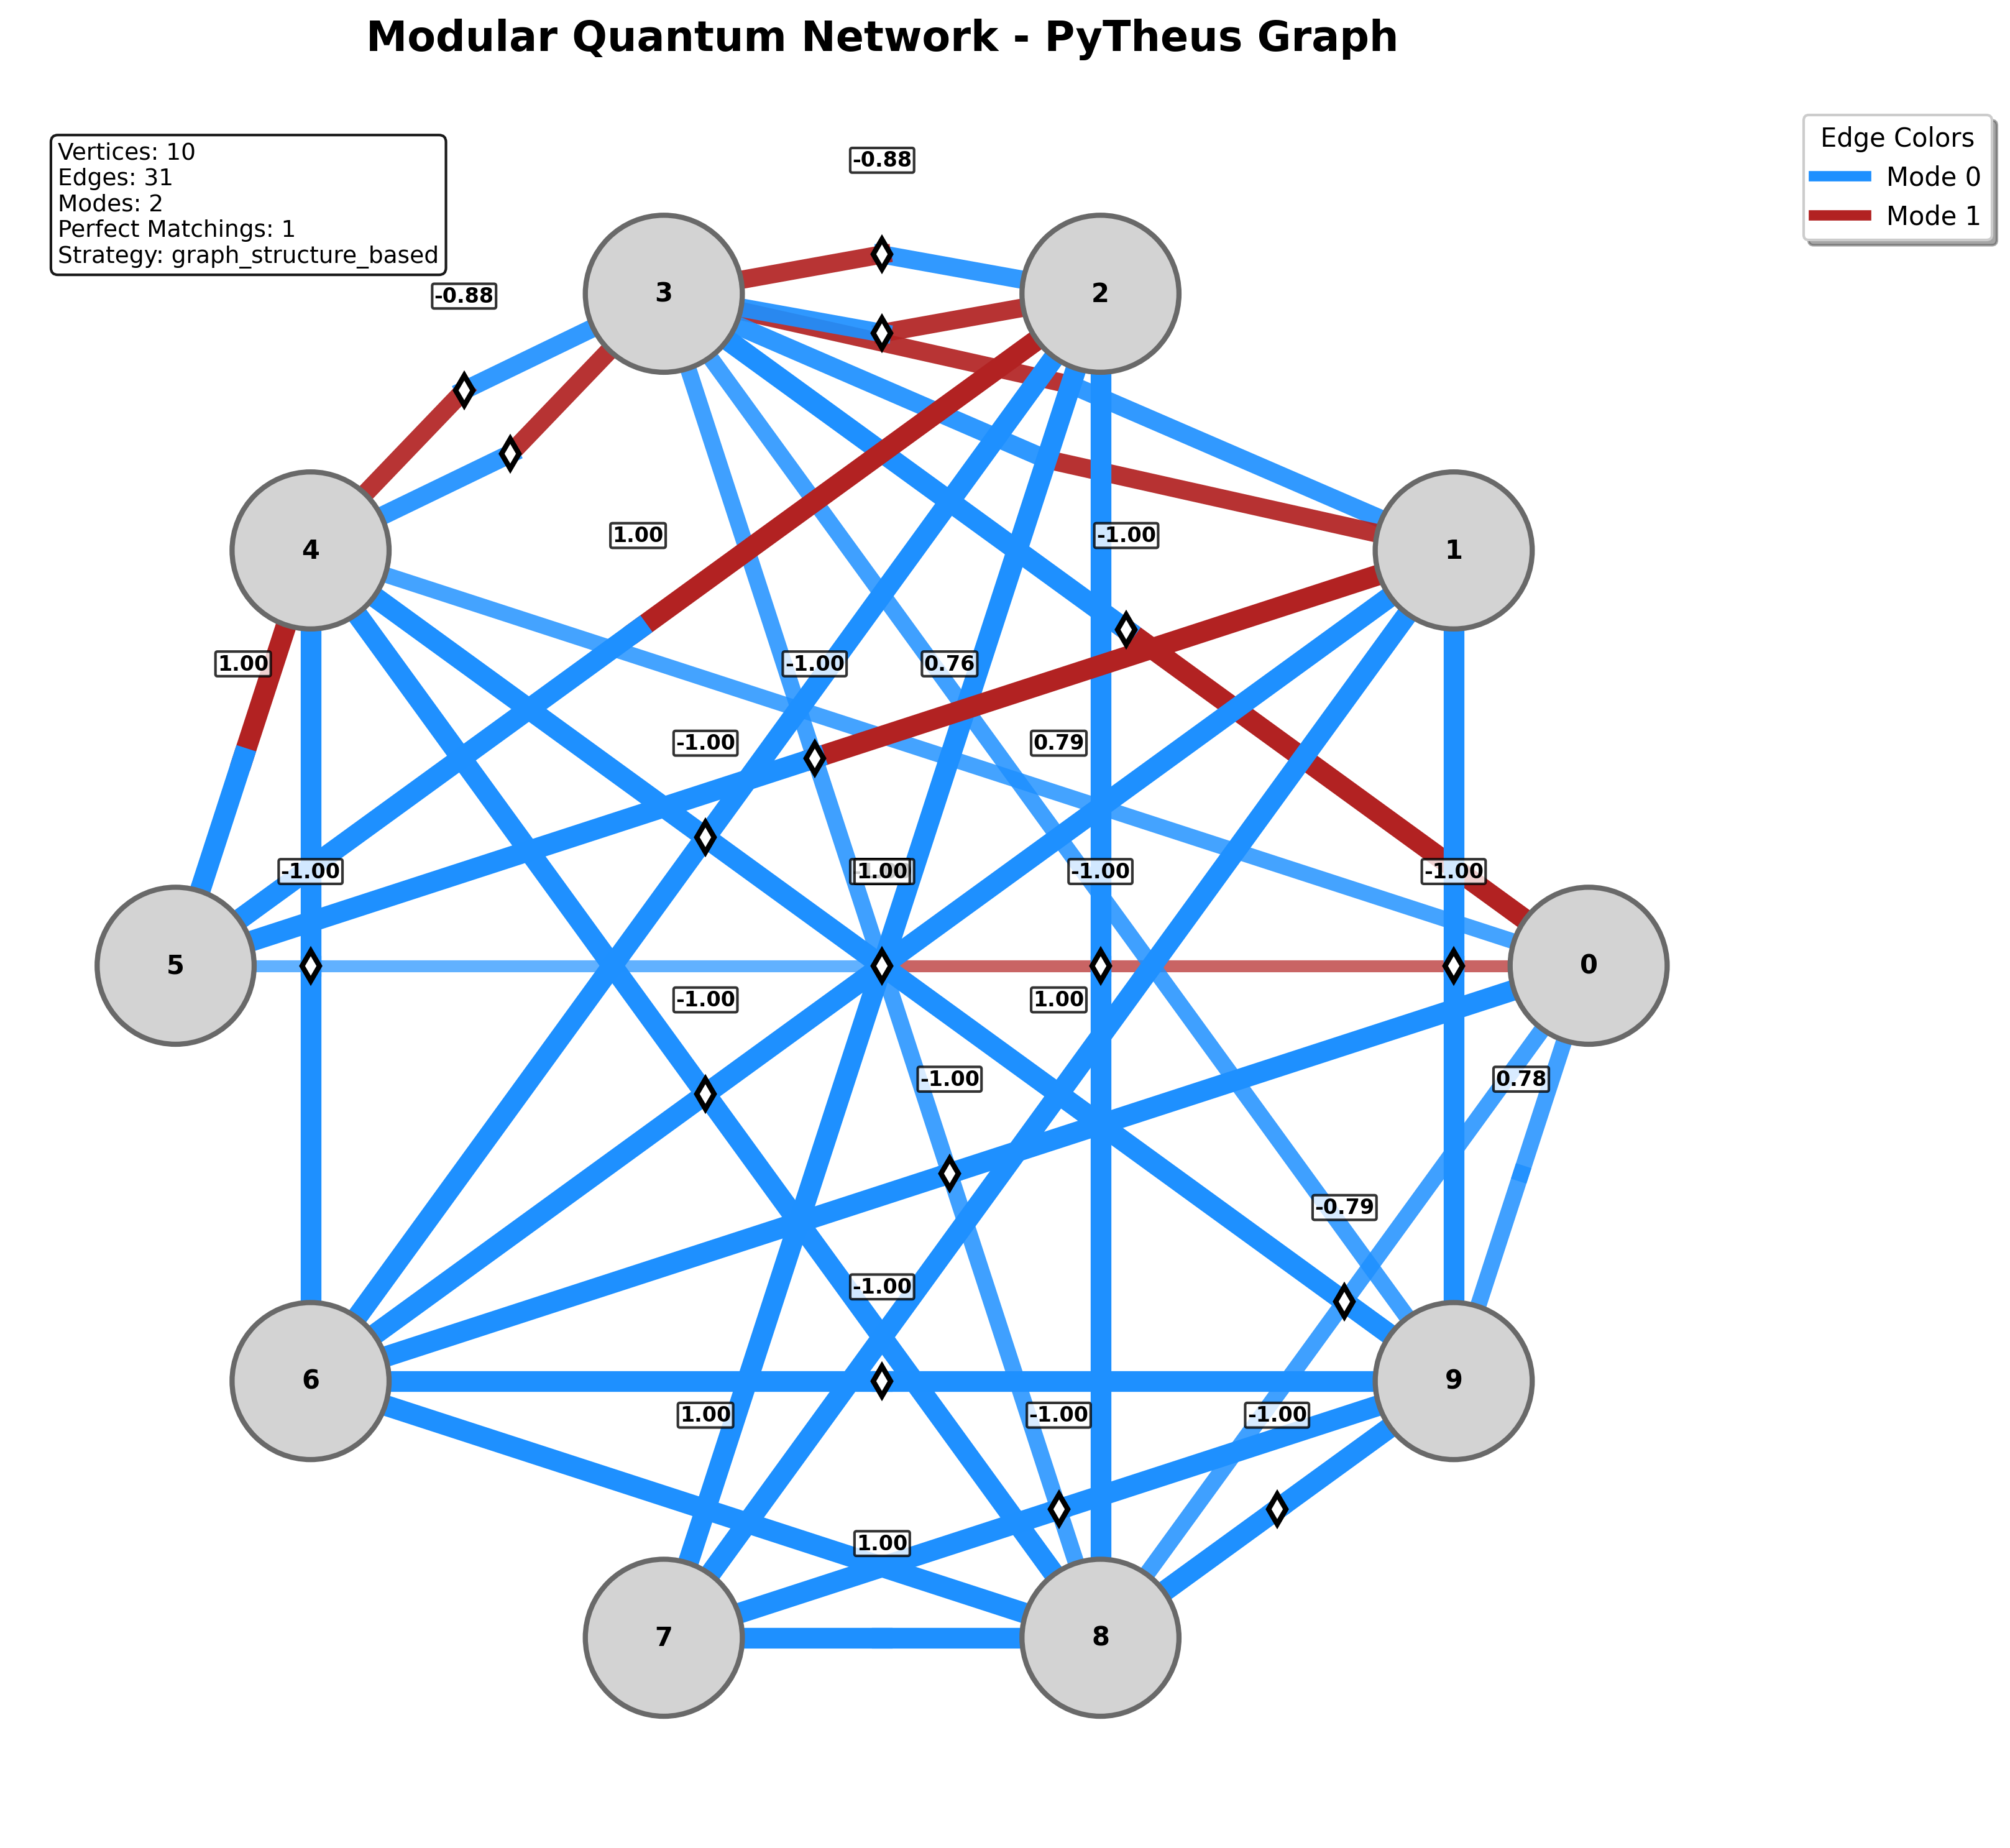
\includegraphics[width=\textwidth]{journal_5node_qkd_native_plot.png}
\caption{Native graph representation showing the 10-vertex, 31-edge architecture with node 3 as the primary hub (degree 9). Edge thickness reflects coupling strength magnitude.}
\label{fig:5node_qkd_native}
\end{subfigure}
\hfill
\begin{subfigure}{0.45\textwidth}
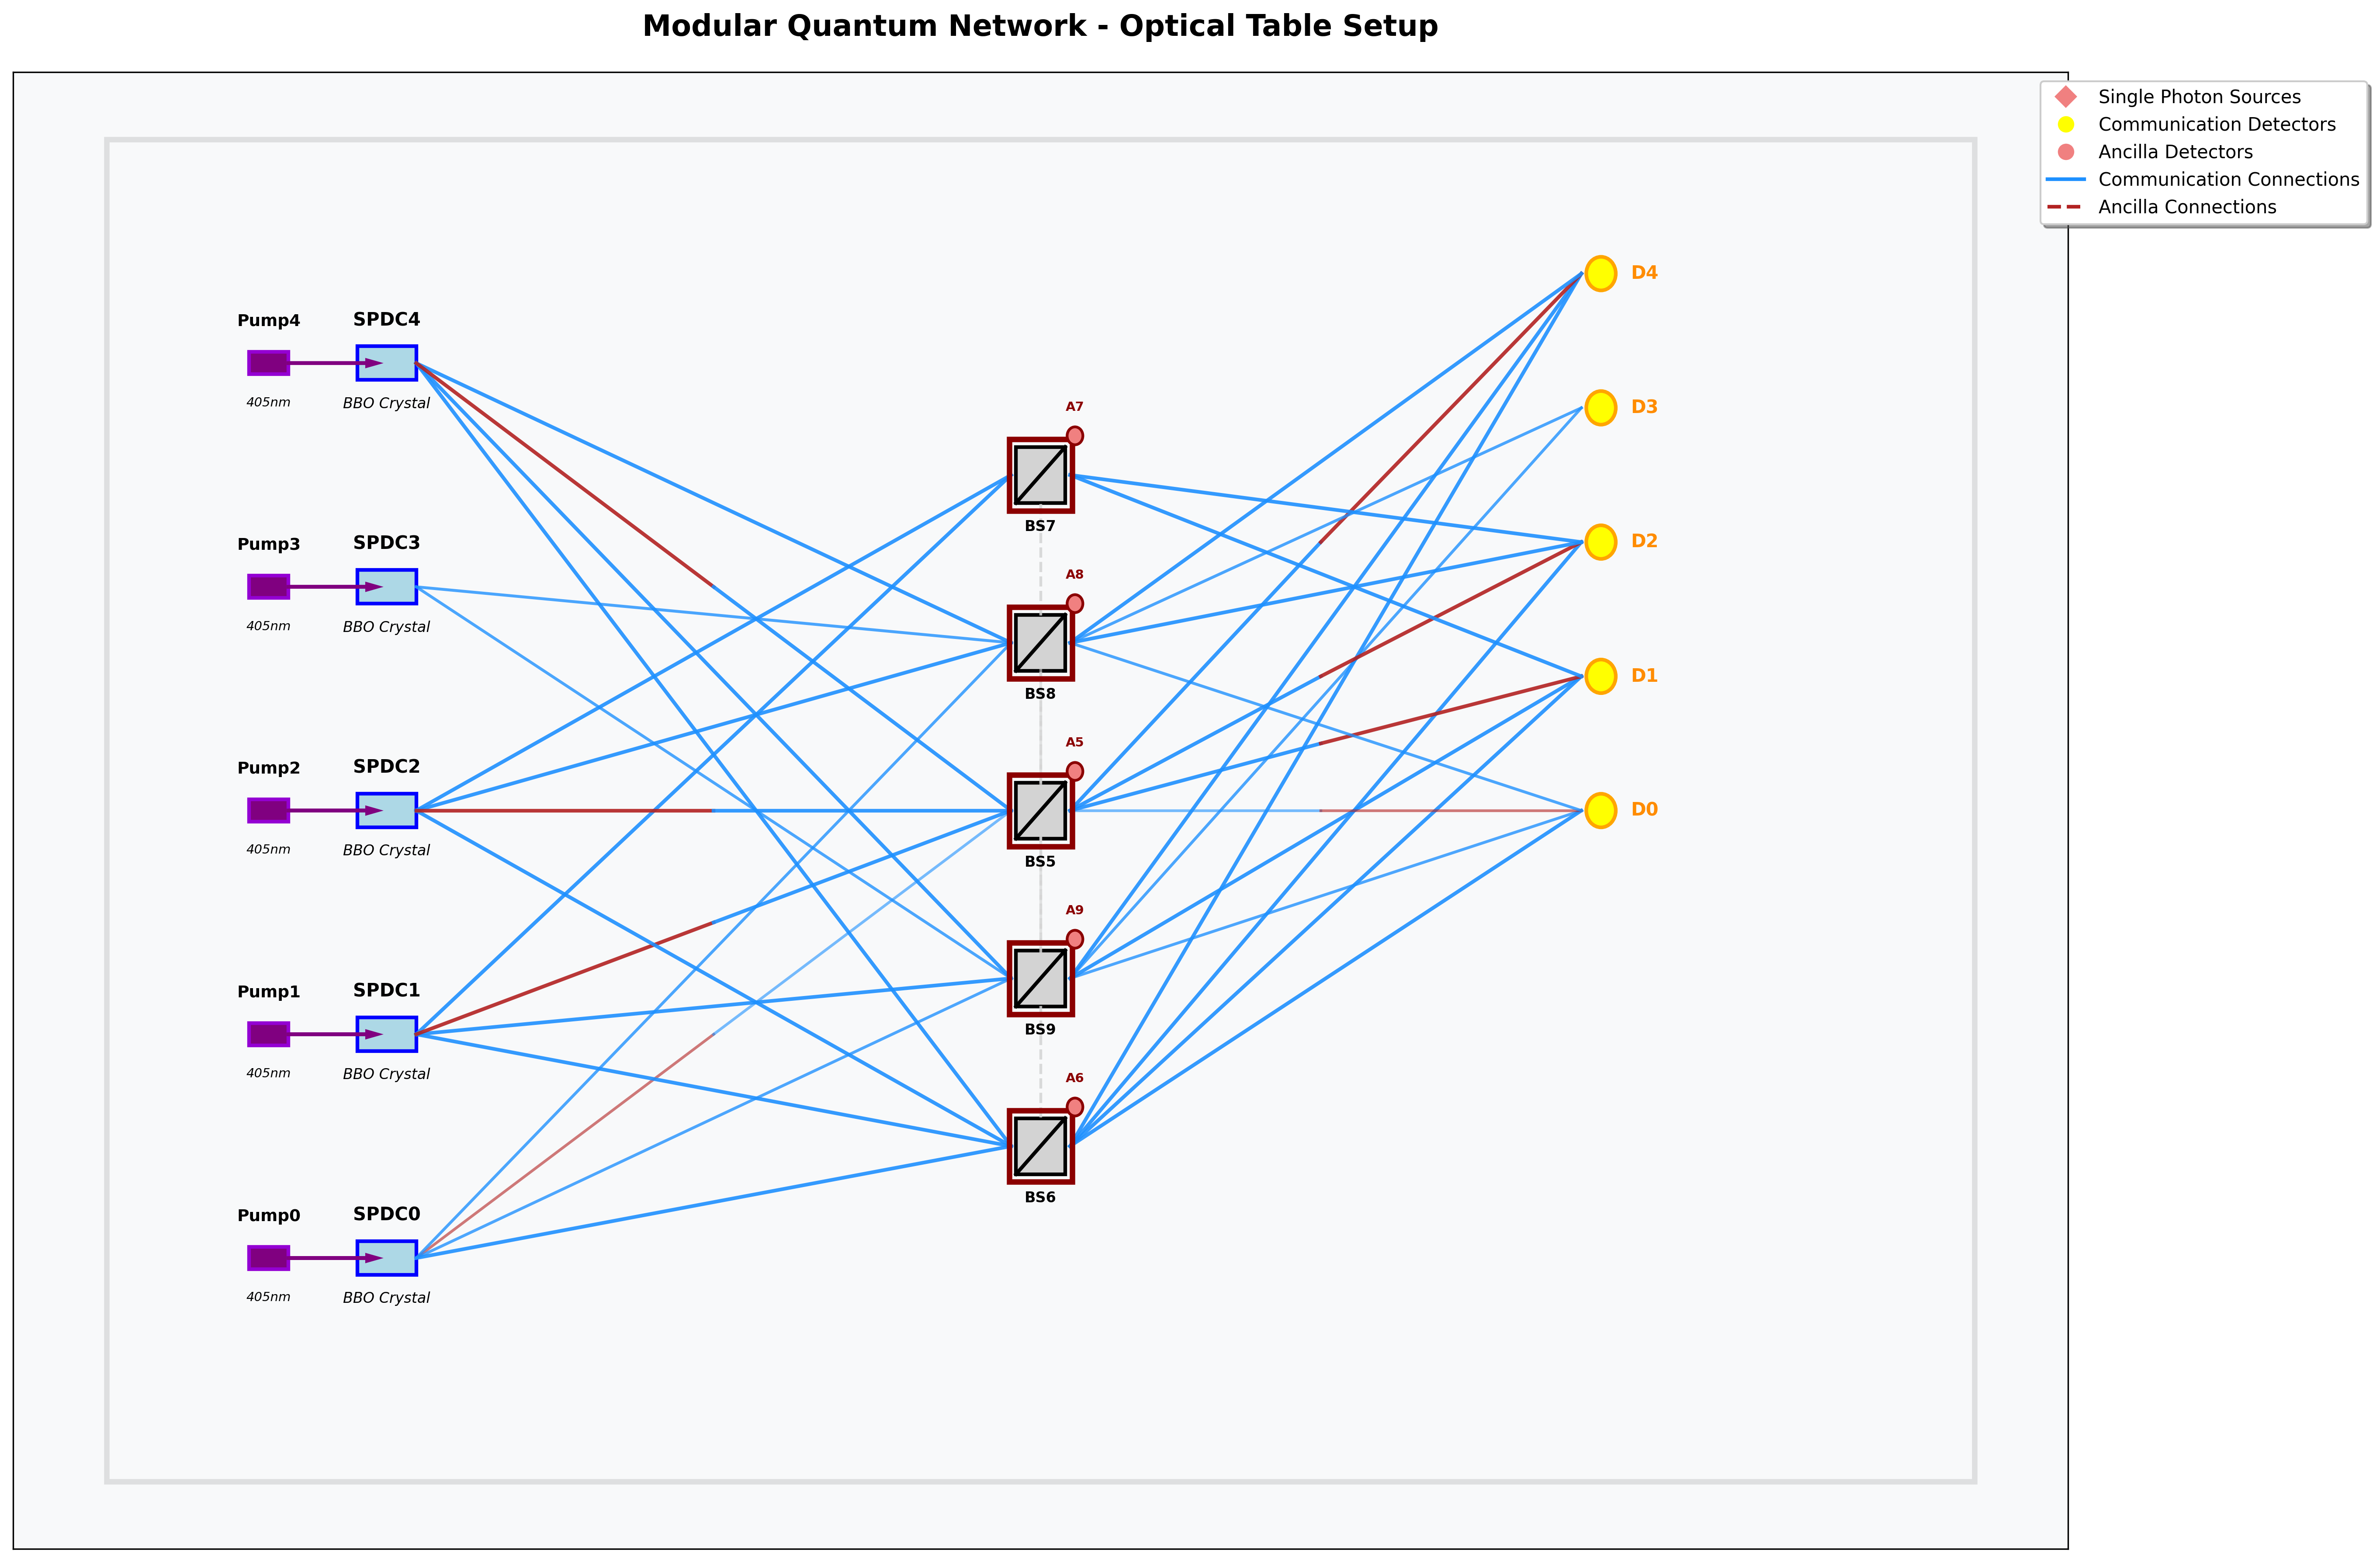
\includegraphics[width=\textwidth]{journal_5node_qkd_optical_table_setup.png}
\caption{Optical table representation showing the dual-role architecture where communication nodes (0-4) serve as both sources and detectors, while ancilla nodes (5-9) function as beam splitters and detectors.}
\label{fig:5node_qkd_optical}
\end{subfigure}
\caption{Five-node QKD network analysis generated by the interpreter from PyTheus optimization output. The native graph (a) reveals the hub-based connectivity with node 3 as the central routing element, while the optical table (b) demonstrates the automated identification of functional roles and physical implementation requirements. Both visualizations maintain consistency between mathematical and physical views of the network architecture.}
\label{fig:5node_qkd_analysis}
\end{figure}

\subsection{Optical Implementation and Signal Routing}

The network's optical implementation employs dual-mode operation using modes 0 and 1, with the interpreter identifying complex coupling patterns across 31 edges. The signal routing analysis reveals a sophisticated distribution of coupling strengths: perfect correlations (±1.0) for critical quantum communication links, and intermediate coupling strengths (0.576 to 0.898) for fine-tuned quantum interference control.

Key optical connections include strong correlations between communication nodes and the central hub (node 3), with coupling strengths like 0.882 (1-3 mode 0→1), -0.883 (3-4 mode 0→1), and -0.884 (2-3 mode 0→1). The ancilla network maintains perfect correlations (±1.0) between multiple pairs: positive correlations (6-8, 7-8) and negative correlations (6-9, 7-9, 8-9), enabling sophisticated measurement and heralding capabilities.

The distributed routing architecture supports the ten-state superposition target through carefully orchestrated optical paths. Communication nodes connect to the central hub node 3 through both modes, while ancilla nodes provide distributed beam splitting and detection. The intermediate coupling strengths (0.576-0.898) enable precise quantum interference control necessary for the balanced superposition of computational basis states, while perfect correlations (±1.0) ensure deterministic measurement outcomes for protocol validation. The native graph representation (Figure~\ref{fig:5node_qkd_native}) clearly shows the hub-based connectivity with edge thickness reflecting coupling strength magnitude, while the optical table layout (Figure~\ref{fig:5node_qkd_optical}) demonstrates the physical implementation of this dual-role architecture. The native graph representation (Figure~\ref{fig:5node_qkd_native}) clearly shows the hub-based connectivity, while the optical table layout (Figure~\ref{fig:5node_qkd_optical}) demonstrates the physical implementation of this dual-role architecture.

\subsection{Ancilla Correlation Network and Heralding Mechanism}

The ancilla correlation network represents one of the most sophisticated aspects of the five-node QKD architecture. The five ancilla detectors (nodes 5-9) maintain strong mutual correlations, with perfect correlations (weight = $\pm 1.0$) between multiple ancilla pairs. These correlations enable a sophisticated heralding mechanism that validates successful quantum state preparation while providing real-time feedback for protocol optimization.

The correlation structure includes five distinct ancilla correlation links: nodes 6-8 and 7-8 exhibit perfect positive correlation (weight = +1.0), while nodes 6-9, 7-9, and 8-9 show perfect anti-correlation (weight = -1.0). This correlation pattern creates a robust error detection mechanism that can identify and correct quantum state preparation failures in real-time, significantly improving the protocol's overall fidelity and security.

The heralding mechanism operates through coincidence detection across the ancilla network. Successful quantum state preparation generates specific correlation patterns across the ancilla detectors, providing a clear signature for valid quantum communication events. Failed state preparation produces different correlation patterns, enabling the protocol to discard corrupted communication attempts and maintain high security standards.

\subsection{Ancilla Network Analysis and Measurement Schemes}

The ancilla correlation network demonstrates sophisticated measurement capabilities through strategic coupling patterns. The five ancilla detectors (nodes 5-9) exhibit strong mutual correlations enabling post-selection and heralding mechanisms. Perfect correlations (±1.0) between specific ancilla pairs create deterministic measurement outcomes:

Key ancilla correlations include:
\begin{itemize}
\item Positive correlations: 6-8 (+1.0), 7-8 (+1.0) - enabling coherent measurement bases
\item Negative correlations: 6-9 (-1.0), 7-9 (-1.0), 8-9 (-1.0) - providing measurement contrast
\item Additional perfect correlations: 4-9 (+1.0), 4-6 (-1.0) - linking communication and ancilla networks
\end{itemize}

These correlation patterns enable sophisticated error detection and quantum state validation. The ancilla network functions as both a beam splitter network (performing optical mixing) and a measurement system (providing heralding capabilities). The perfect correlations (±1.0) ensure deterministic outcomes for specific photon patterns, while the distributed architecture maintains quantum coherence across the multi-party communication protocol.

The ancilla measurement scheme operates through coincidence detection across the five ancilla detectors, providing real-time feedback on quantum state preparation success. This enables the protocol to post-select valid communication events while discarding preparation failures, significantly improving overall fidelity and security.

\subsection{Performance Characteristics and Implementation Feasibility}

The five-node QKD network demonstrates remarkable performance characteristics that position it for practical implementation. The network's 31-edge architecture, while complex, remains within the implementation capabilities of current optical quantum technology. The dual-mode operation (modes 0 and 1) can be implemented using standard optical components with mode-division multiplexing capabilities.

The network's scalability potential stems from its distributed architecture and dual-role node design. The hub-based structure with node 3 as the primary hub provides efficient routing while avoiding centralized bottlenecks. The dual-role ancilla nodes provide the flexibility necessary for protocol adaptation, functioning both as beam splitters and measurement devices.

The two-photon target state structure enables implementation using standard quantum optical sources, ensuring compatibility with existing quantum communication infrastructure. The sophisticated correlation structure provides the foundation for extending the network to additional parties while maintaining security guarantees through the balanced ten-state superposition and robust ancilla measurement schemes.

\subsection{Hub-Based Network Architecture}

The network architecture centers around node 3 as the primary hub with degree 9, providing efficient routing for the five-party quantum communication protocol. The hub-based design enables complex quantum state generation through strategic coupling patterns between communication nodes and the central hub.

\textbf{Communication Node Connections}: The five communication nodes (0-4) connect to the central hub through both optical modes with specific coupling strengths:
\begin{itemize}
\item Node 0 connections: 0-3 (mode 1→0, weight -1.0), 0-5 (mode 1→0, weight 0.576), 0-4 (mode 0→0, weight 0.760), 0-9 (mode 0→0, weight 0.785), 0-8 (mode 0→0, weight -0.793), 0-6 (mode 0→0, weight -1.0)
\item Node 1 connections: 1-3 (mode 0→1, weight 0.882), 1-3 (mode 1→0, weight 0.898), 1-9 (mode 0→0, weight -1.0), 1-7 (mode 0→0, weight 1.0), 1-6 (mode 0→0, weight 1.0), 1-5 (mode 1→0, weight -1.0)
\item Node 2 connections: 2-3 (mode 0→1, weight -0.884), 2-3 (mode 1→0, weight -0.893), 2-8 (mode 0→0, weight -1.0), 2-7 (mode 0→0, weight -1.0), 2-6 (mode 0→0, weight -1.0), 2-5 (mode 1→0, weight 1.0)
\item Node 4 connections: 3-4 (mode 0→1, weight -0.883), 3-4 (mode 1→0, weight -0.895), 4-8 (mode 0→0, weight -0.997), 4-9 (mode 0→0, weight 1.0), 4-6 (mode 0→0, weight -1.0), 4-5 (mode 1→0, weight 1.0)
\end{itemize}

\textbf{Ancilla Network Integration}: The ancilla detectors (nodes 5-9) maintain perfect correlations (±1.0) enabling sophisticated measurement capabilities:
\begin{itemize}
\item Perfect positive correlations: 6-8 (+1.0), 7-8 (+1.0), 4-9 (+1.0), 1-7 (+1.0), 1-6 (+1.0), 2-5 (+1.0), 4-5 (+1.0)
\item Perfect negative correlations: 6-9 (-1.0), 7-9 (-1.0), 8-9 (-1.0), 1-9 (-1.0), 2-8 (-1.0), 2-7 (-1.0), 2-6 (-1.0), 4-8 (-0.997), 4-6 (-1.0), 0-8 (-0.793), 0-6 (-1.0), 1-5 (-1.0)
\end{itemize}

This hub-based architecture enables the complex ten-state superposition target through coordinated quantum interference across both optical modes while maintaining robust ancilla measurement capabilities. The complete network structure is visualized in Figure~\ref{fig:5node_qkd_analysis}, which shows both the native graph representation and the corresponding optical table setup.

\subsection{Interpreter Analysis Pipeline}

Our interpreter's analysis of the five-node network demonstrates the sophisticated multi-stage processing pipeline in action. The system begins by parsing the PyTheus graph structure, which contains 31 edges represented as tuples \texttt{(v1, v2, mode1, mode2)} with associated coupling weights across the 10-vertex network.

\textbf{Structural Analysis Phase}: The interpreter employs \texttt{\_compute\_vertex\_degrees} to analyze connectivity patterns, identifying node 3 as the primary hub with degree 9. The \texttt{\_analyze\_connectivity} method using NetworkX computes comprehensive graph metrics: density (0.6222), clustering coefficient (0.4905), diameter (2), and identifies 24 triangle motifs and 89 square motifs indicating rich local connectivity.

\textbf{Configuration Integration}: The system parses PyTheus configuration data, extracting \texttt{out\_nodes} [0,1,2,3,4] as communication parties, \texttt{anc\_detectors} [5,6,7,8,9] as ancilla detectors, and the ten-state \texttt{target\_state} superposition. The interpreter's \texttt{\_analyze\_quantum\_state} method validates the balanced two-photon state structure.

\textbf{Functional Role Inference}: The interpreter correctly identifies all nodes 0-4 as both sources and detectors based on the \texttt{out\_nodes} configuration, recognizing the dual-role architecture. The \texttt{\_identify\_beam\_splitter\_\\nodes} method identifies nodes [6,9,5,8,7] as beam splitters, while \texttt{\_identify\_ancilla\_nodes} uses the \texttt{anc\_detectors} configuration to identify the ancilla network.

\textbf{Implementation Strategy Determination}: The \texttt{\_determine\_implementation\_strategy} method identifies this as a complex network requiring heralding, with 5 sources, 10 detectors, 5 beam splitters, and 5 ancillas. The system determines that the dual-mode operation (modes 0,1) and perfect correlations (±1.0) require sophisticated optical implementation.

\textbf{Optical Routing Analysis}: The interpreter generates routing through \texttt{\_build\_connection\_map} preserving the hub-based architecture with node 3 as the central routing element. The system implements dual-mode visualization supporting both (0,0) and (1,0) mode connections while maintaining the coupling strength hierarchy from perfect correlations (±1.0) to intermediate values (0.576-0.898).

\subsection{Visualization Generation Results}

The interpreter's dual visualization approach produces coordinated outputs that reveal different aspects of the network architecture:

\textbf{Native Graph Output}: The \texttt{plot\_native\_graph} method recreates PyTheus's visual style using circular vertex layouts, color-coded edges following the standard color scheme (dodgerblue for mode 0, firebrick for mode 1), and edge thickness proportional to coupling strength magnitudes. The system properly visualizes the 10-vertex, 31-edge architecture with node 3 as the primary hub.

\textbf{Optical Table Translation}: The \texttt{plot\_optical\_table\_setup} method automatically selects \texttt{\_plot\_general\_spdc\_optical\_table} for this network type, recognizing the dual-role architecture where communication nodes serve as both sources and detectors. The system positions the hub node 3 centrally while distributing ancilla beam splitter-detectors (5-9) appropriately.

\textbf{Consistency Validation}: The system employs \texttt{\_analyze\_connectivity} to verify the non-bipartite graph structure (bipartite: false) and validates that the optical routing matches the hub-based architecture. The \texttt{generate\_analysis\_report} method produces comprehensive validation reports confirming the complex network characteristics: 24 triangles, 89 squares, density 0.6222, and diameter 2.

\section{Target State Analysis}

The target quantum state represents a crucial element linking network architecture to operational requirements. Understanding the relationship between PyTheus-optimized network structures and their intended quantum states provides essential insights for validation and implementation. Our interpreter includes comprehensive analysis capabilities for target quantum states, enabling systematic evaluation of architecture-state compatibility and revealing design principles that guide network optimization.

\subsection{Automated State Structure Analysis}

Our interpreter includes automated analysis capabilities for target quantum states specified in PyTheus configurations. For the five-node network, the interpreter analyzes the target state structure and its relationship to the discovered architecture.

The target state consists of a superposition of computational basis states with specific photon number and distribution properties. Our interpreter automatically extracts key state properties through the \texttt{\_analyze\_quantum\_state} method:

\begin{align}
\ket{\psi_{\text{target}}} &= \frac{1}{\sqrt{N}} \sum_{i} \ket{\text{basis}_i}
\end{align}

where $N$ is the number of basis states and each $\ket{\text{basis}_i}$ represents a computational basis state.

\subsection{State-Architecture Compatibility}

The interpreter performs automated compatibility analysis between the target state and the identified network architecture through integrated validation methods:

\textbf{Photon Number Analysis}: The \texttt{\_analyze\_quantum\_state} method extracts photon number patterns from target states and validates compatibility with identified source configurations through \texttt{\_identify\_actual\_sources}.

\textbf{Connectivity Requirements}: The \texttt{\_analyze\_connectivity} method confirms that graph connectivity supports the correlations required by the target state structure, validating network topology against quantum state requirements.

\textbf{Ancilla Role Validation}: The \texttt{\_identify\_ancilla\_nodes} method verifies that identified ancilla elements can support the post-selection or measurement requirements implied by the target state, ensuring protocol compatibility.

This automated analysis through the \texttt{analyze\_network\_structure} method provides comprehensive validation that the PyTheus optimization has successfully identified an architecture capable of generating the desired quantum state.

\section{Validation Using Existing PyTheus Examples}

To validate the interpreter's generality and robustness, we systematically applied it to three well-established PyTheus examples representing different classes of quantum networks. These examples serve as important benchmarks for confirming that the interpreter can handle diverse architectures without requiring manual parameter adjustment.

\subsection{W4 State Generation Network}

The W4 state represents a canonical example of symmetric multiparty entanglement implemented using single-photon sources. The PyTheus W4 example demonstrates the generation of the 4-party W state $|W\rangle = (|0001\rangle + |0010\rangle + |0100\rangle + |1000\rangle)/2$ through an optimized linear optical network.

The interpreter analysis revealed an 8-vertex, 10-edge bipartite network with moderate density (0.3571) and diameter 4, utilizing four single-photon sources (nodes 4, 5, 6, 7) to generate entanglement across four communication parties (nodes 0, 1, 2, 3). The network architecture exhibits a hub-and-spoke structure with node 5 serving as a central hub (degree 4), while maintaining the distributed connectivity necessary for W-state generation. The network demonstrates zero clustering coefficient (0.0000) characteristic of bipartite graphs, with a mean degree of 2.50 across all nodes.

The optical implementation employs dual-mode operation (modes 0 and 1) with perfect coupling coefficients (±1.0), creating the quantum interference patterns necessary for symmetric multiparty entanglement. Key optical connections include positive couplings (1-6, 2-5, 2-6, 1-4, 1-5) and negative couplings (3-4, 3-7, 0-7, 0-5, 3-5), with the hub node 5 providing critical connectivity across both optical modes. The network exhibits 3 square motifs and 3 star motifs, with no triangular structures due to its bipartite nature. The interpreter correctly identified this as a pure single-photon source network with no beam splitters or ancillas, confirming the network's reliance on direct optical routing for quantum state generation. The complete network structure is shown in Figure~\ref{fig:w4_analysis}.

\begin{figure}[htbp]
\centering
\begin{subfigure}{0.45\textwidth}
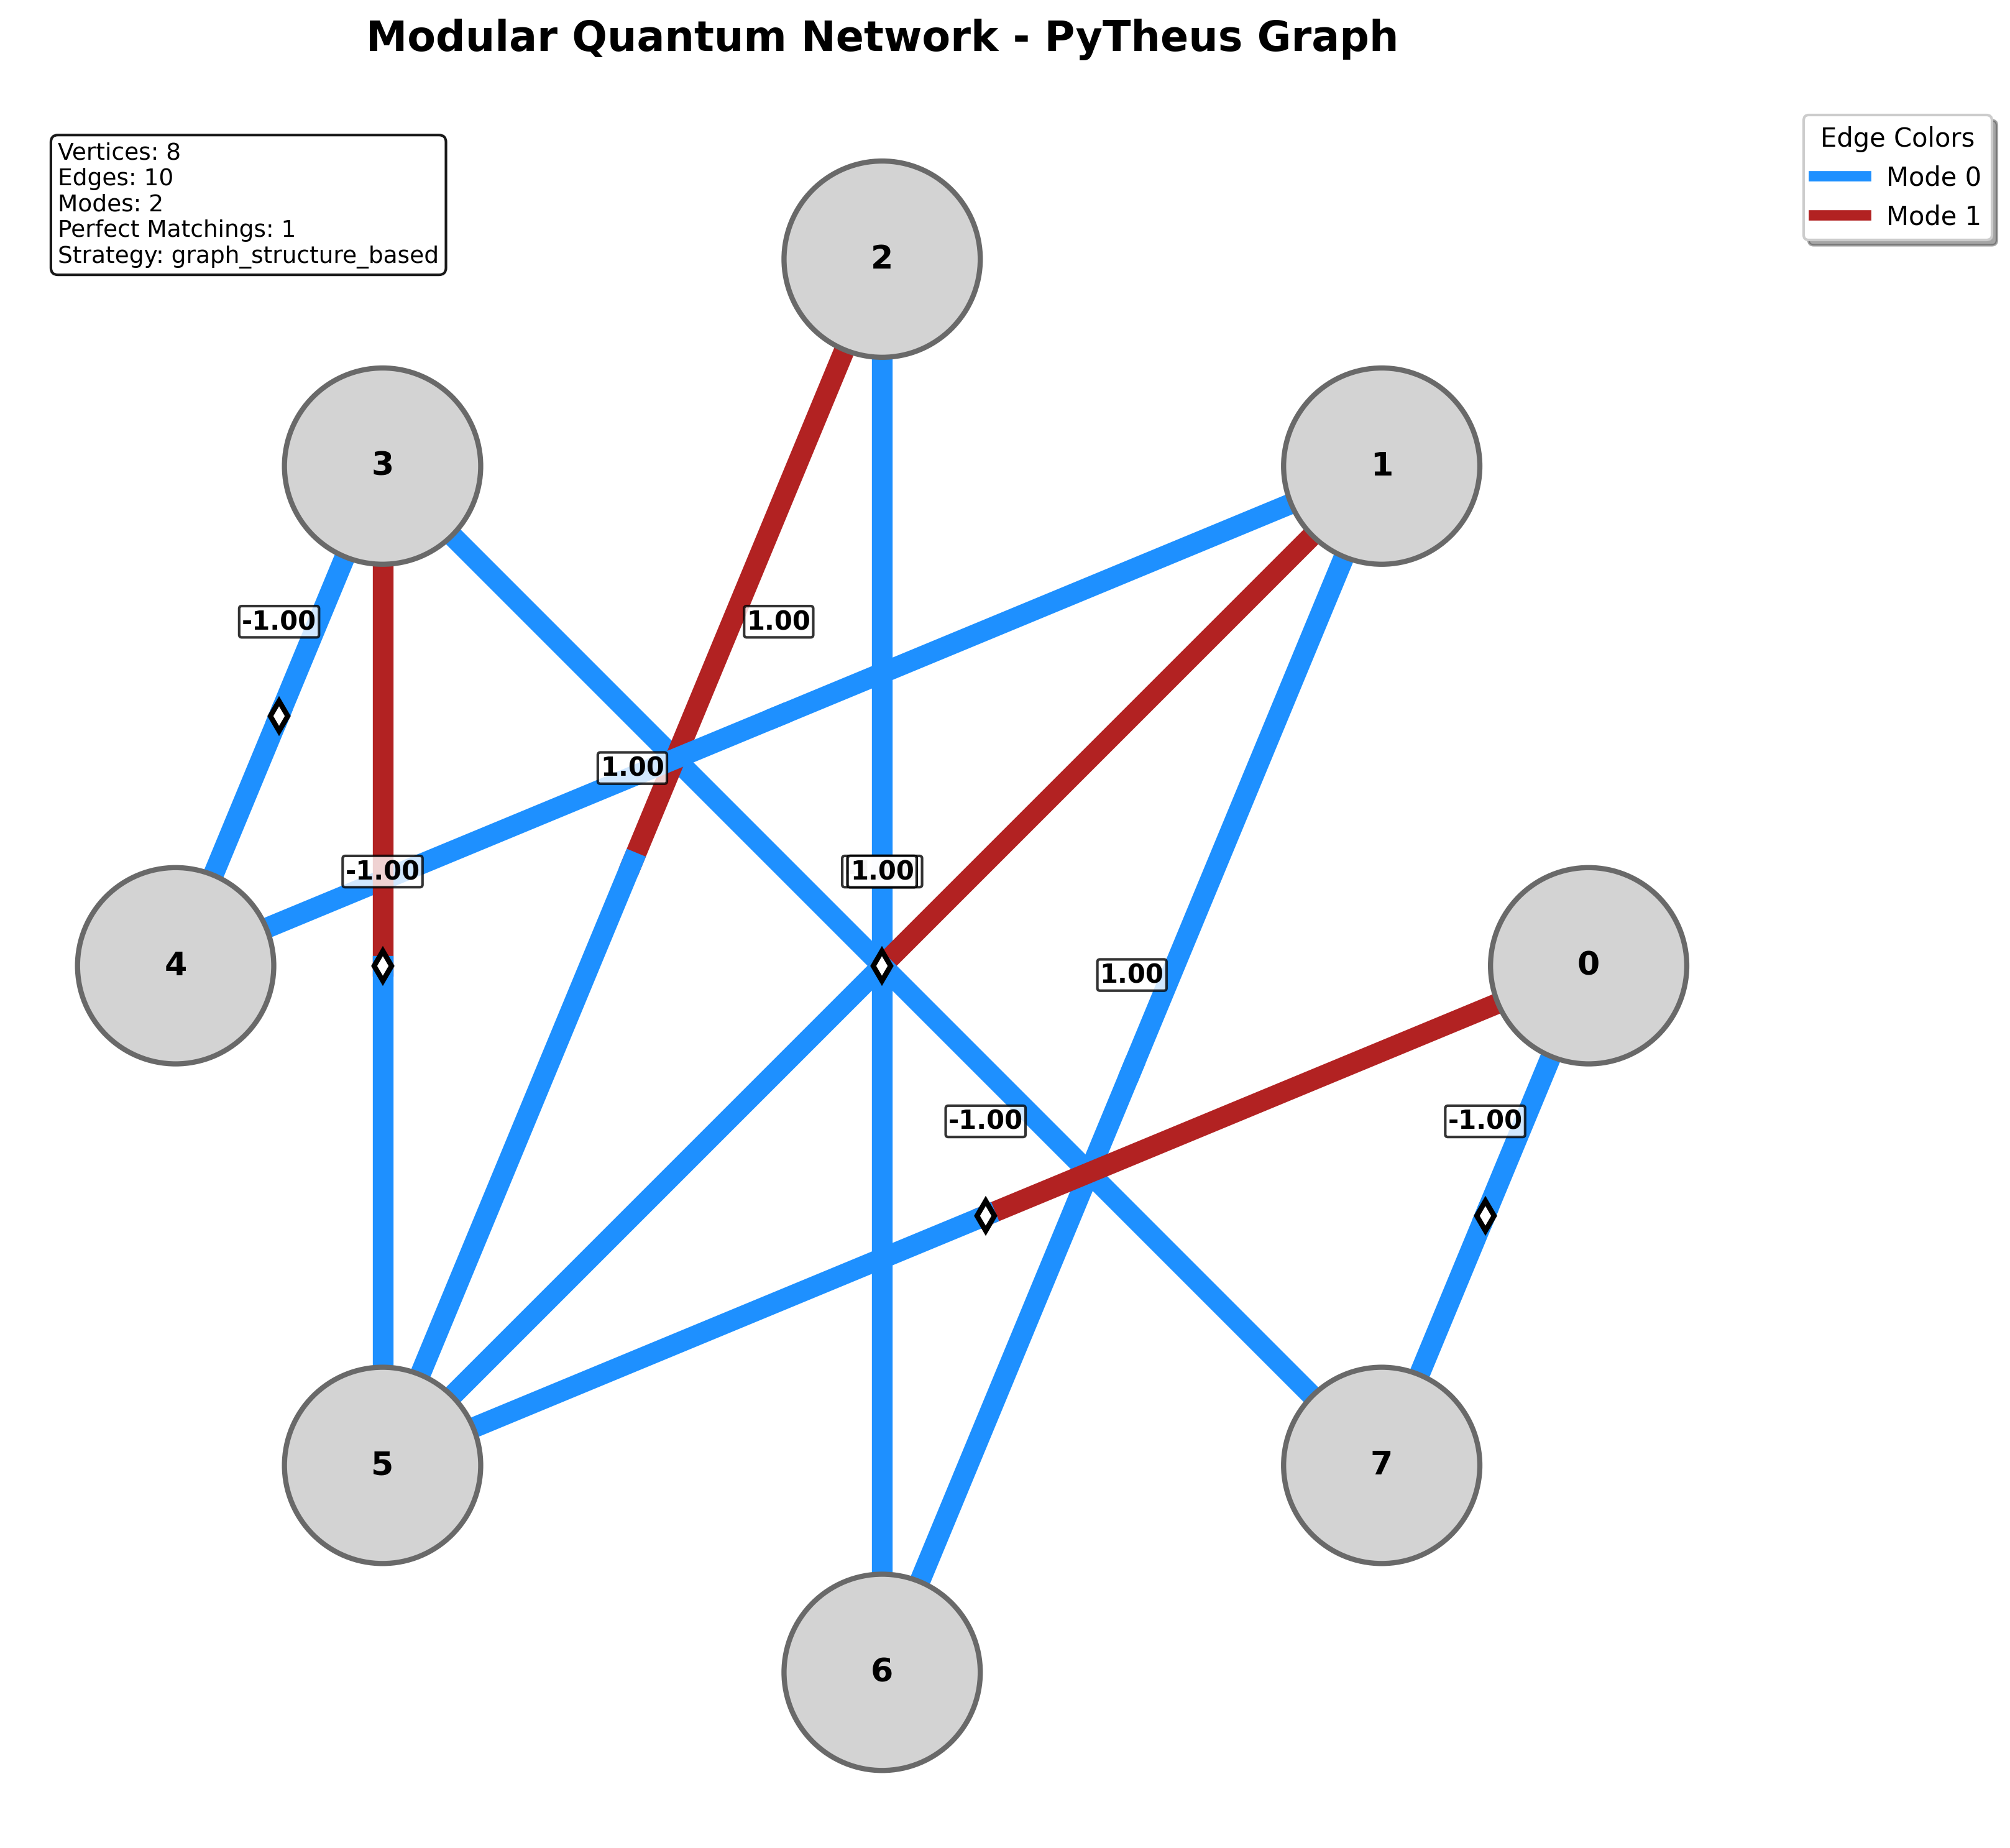
\includegraphics[width=\textwidth]{journal_w4_state_native_plot.png}
\caption{Native graph showing 8-vertex bipartite structure with hub node 5 (degree 4) and distributed single-photon sources (nodes 4,5,6,7).}
\end{subfigure}
\hfill
\begin{subfigure}{0.45\textwidth}
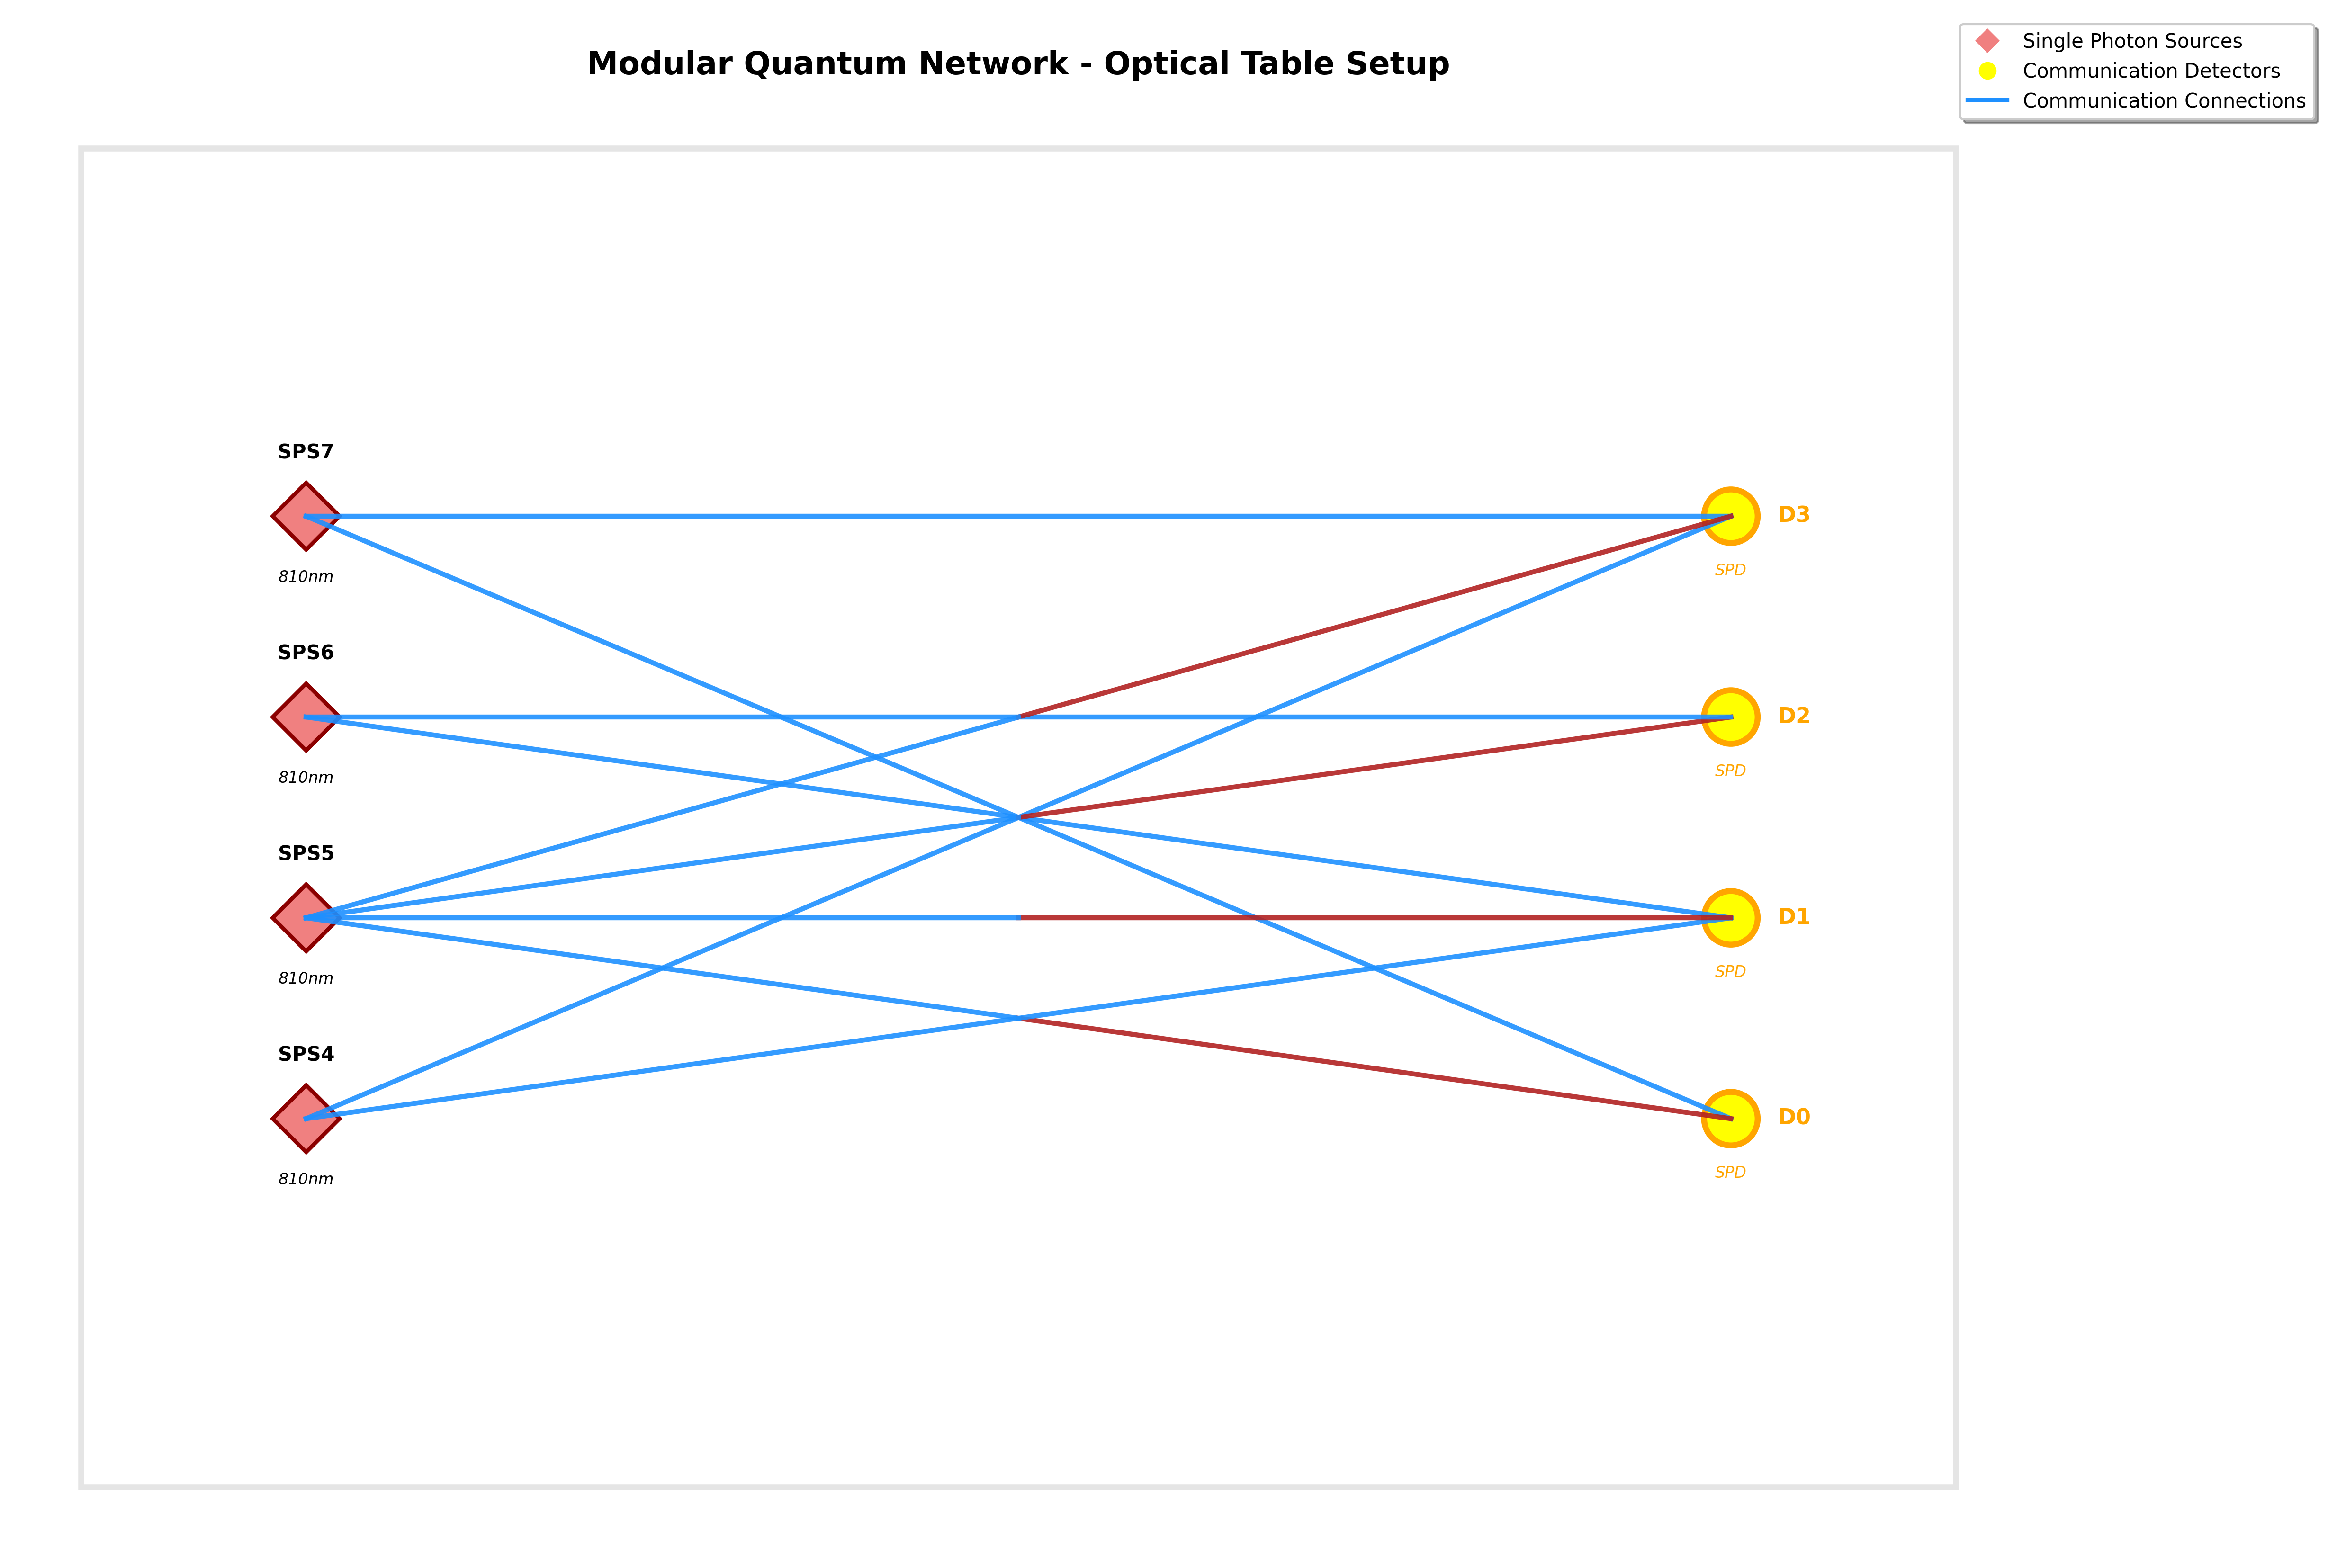
\includegraphics[width=\textwidth]{journal_w4_state_optical_table_setup.png}
\caption{Optical table demonstrating direct optical routing without beam splitters, enabling symmetric 4-party W state generation.}
\end{subfigure}
\caption{W4 state generation network analysis showing symmetric 4-party architecture with distributed single-photon sources and direct optical routing for multiparty entanglement.}
\label{fig:w4_analysis}
\end{figure}

\subsection{Heralded Bell State Preparation}

The heralded Bell state example represents a sophisticated 2-party network that demonstrates the interpreter's capability to analyze networks with ancilla-based heralding mechanisms. This network generates high-fidelity Bell states through post-selection enabled by ancilla measurements.

The interpreter identified an 8-vertex, 12-edge bipartite network with density 0.4286 and diameter 4, employing four single-photon sources (nodes 2, 3, 4, 5) to create Bell state correlations between two communication parties (nodes 0, 1). The network incorporates two ancilla detectors (nodes 6, 7) that function as hub nodes, enabling heralding functionality through post-selection of successful Bell state generation events. The network exhibits zero clustering coefficient (0.0000) characteristic of bipartite structures, with a mean degree of 3.00 and 10 square motifs indicating substantial local connectivity.

The optical routing analysis revealed sophisticated interference patterns with two distinct coupling regimes: strong primary couplings (±1.0) for the communication channels (0-4, 1-5, 1-2, 0-3) and weak ancilla couplings (±0.1) for the heralding connections. The ancilla nodes maintain weak coupling to all four sources (2-7, 3-7, 4-7, 5-7 with weights 0.1, 0.1, 0.1, -0.1 respectively, and 3-6, 5-6, 2-6, 4-6 with weights 0.1, 0.1, 0.1, -0.1 respectively), creating the quantum interference necessary for Bell state generation while providing the non-destructive measurement capability required for heralding.

The interpreter correctly classified this architecture as a single-photon source network with ancilla heralding, distinguishing it from SPDC-based approaches while recognizing the critical dual-mode operation (modes 0 and 1) and the hub-based connectivity pattern that enables the protocol's probabilistic operation through post-selection. The network architecture is illustrated in Figure~\ref{fig:bell_analysis}.

\begin{figure}[htbp]
\centering
\begin{subfigure}{0.45\textwidth}
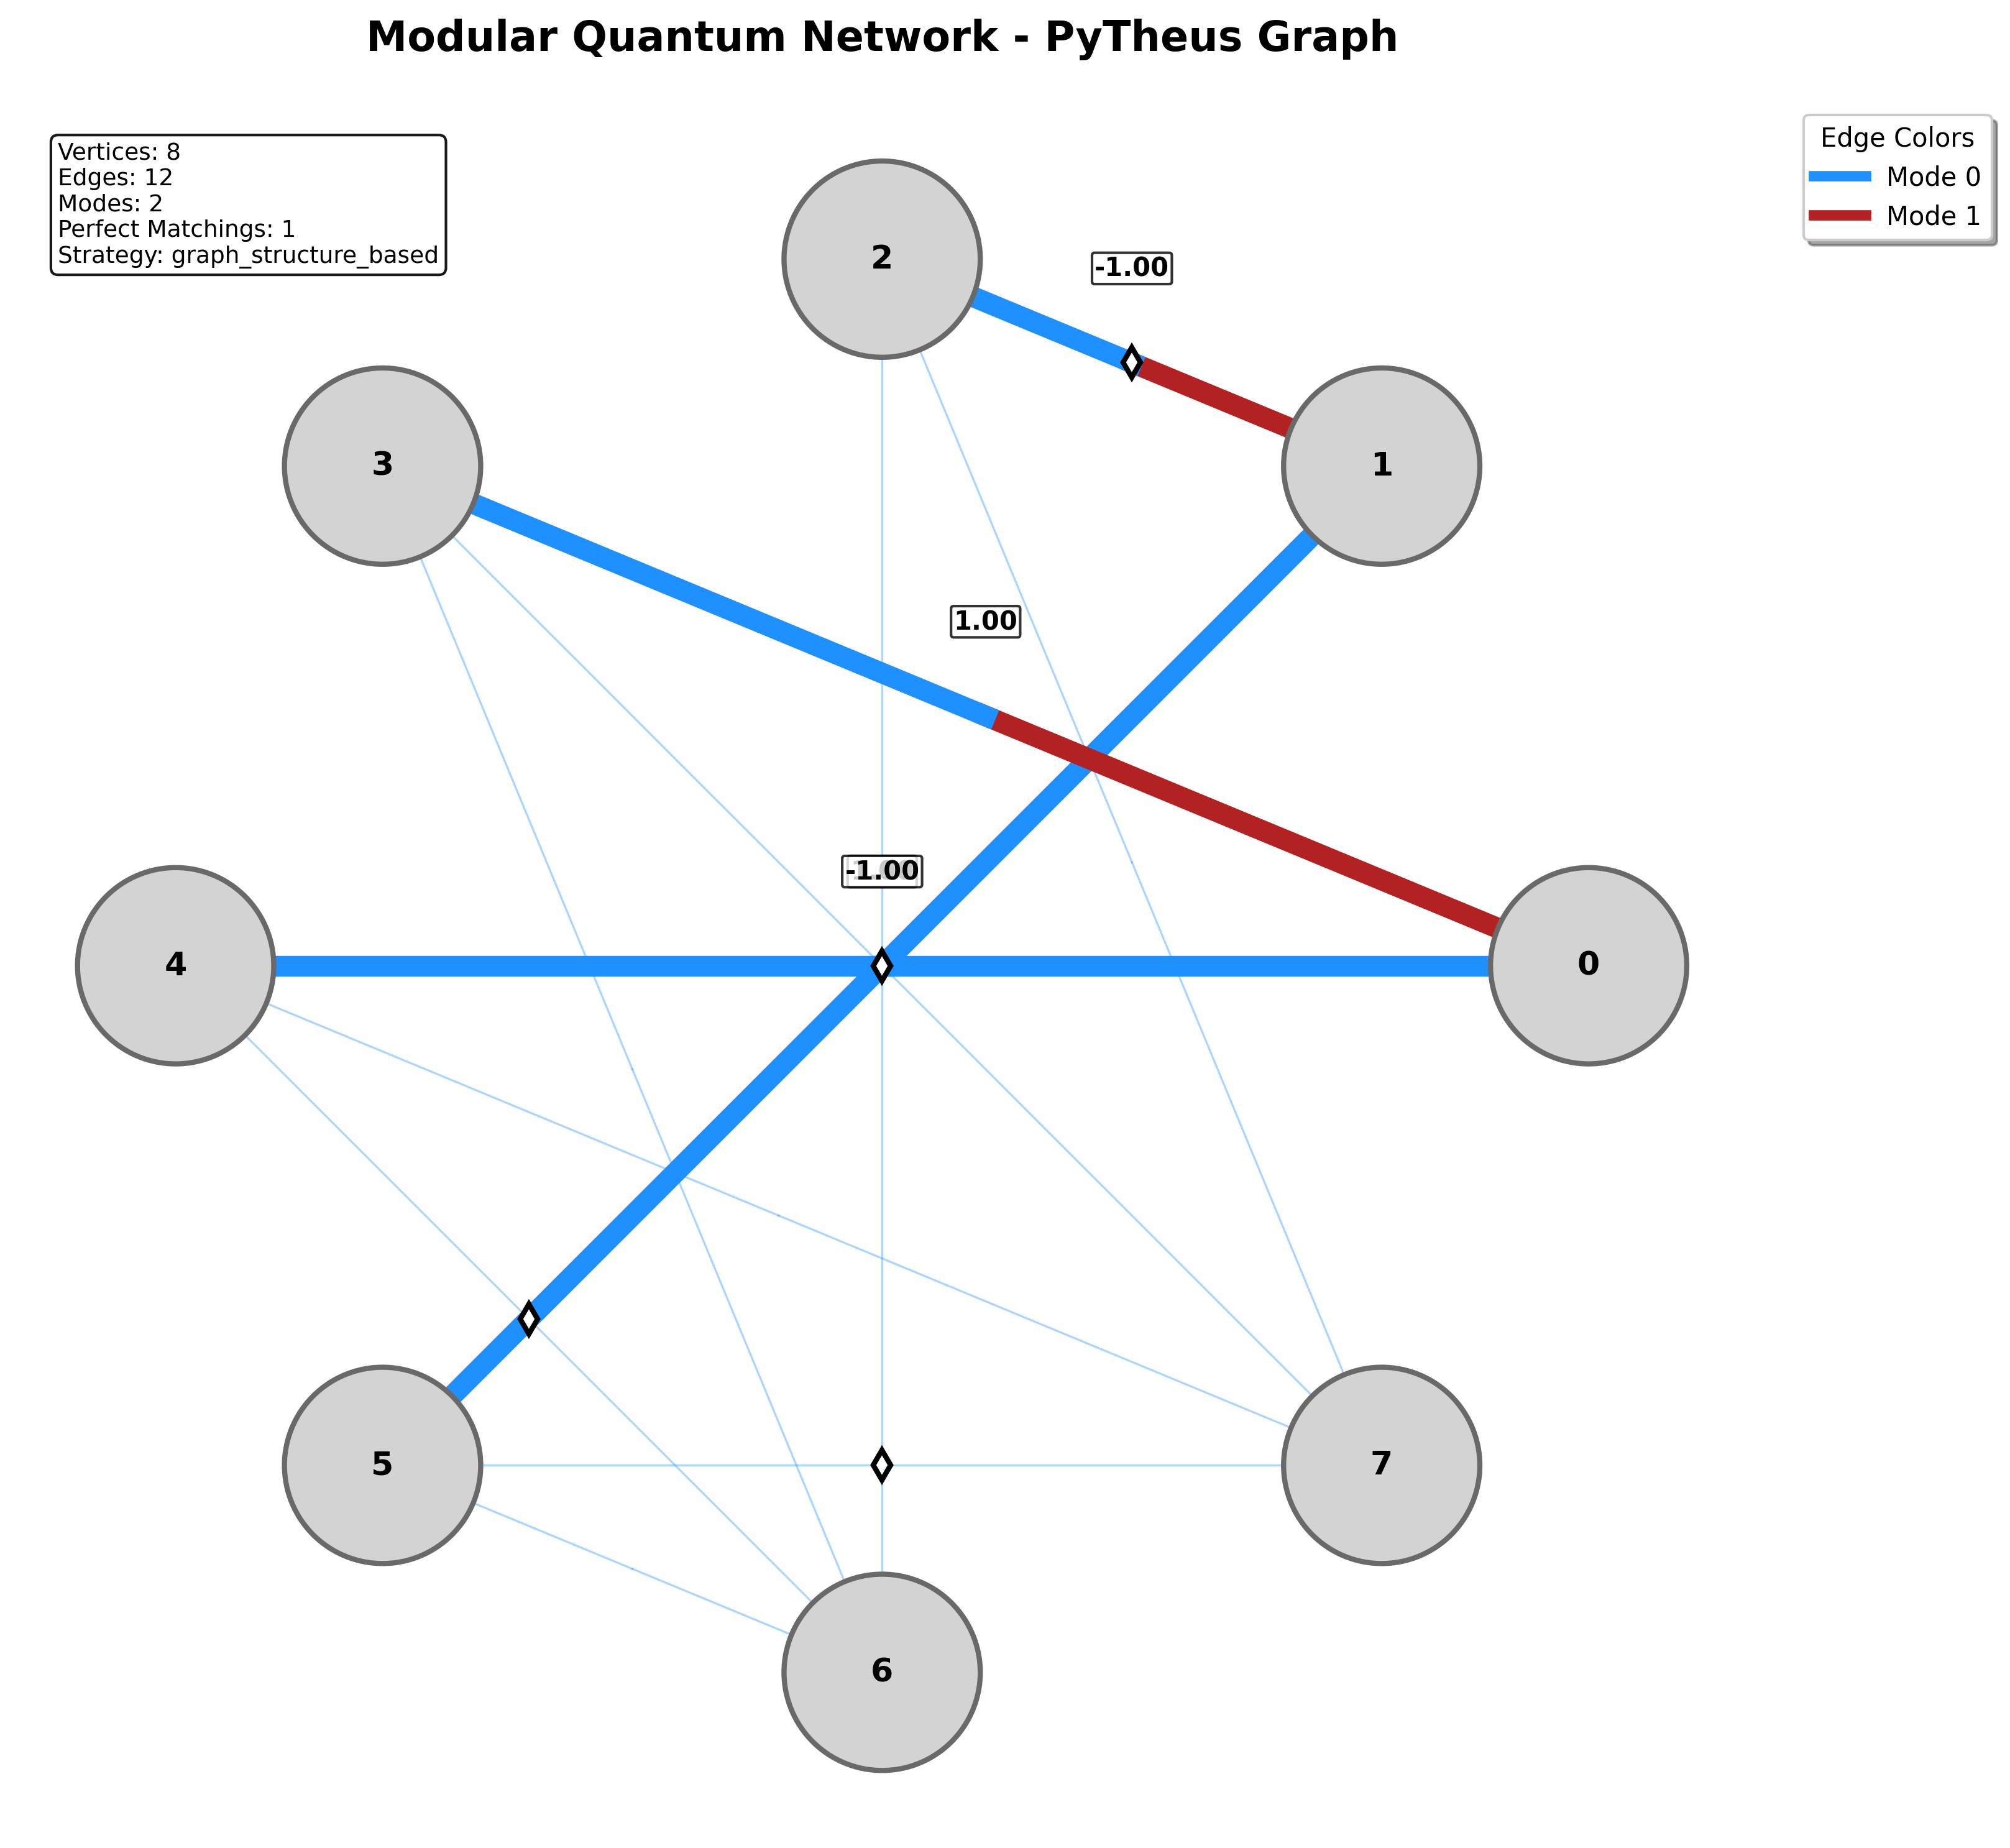
\includegraphics[width=\textwidth]{journal_heralded_bell_native_plot.png}
\caption{Native graph showing 8-vertex bipartite network with ancilla hubs (nodes 6,7) enabling heralding through weak couplings (±0.1).}
\end{subfigure}
\hfill
\begin{subfigure}{0.45\textwidth}
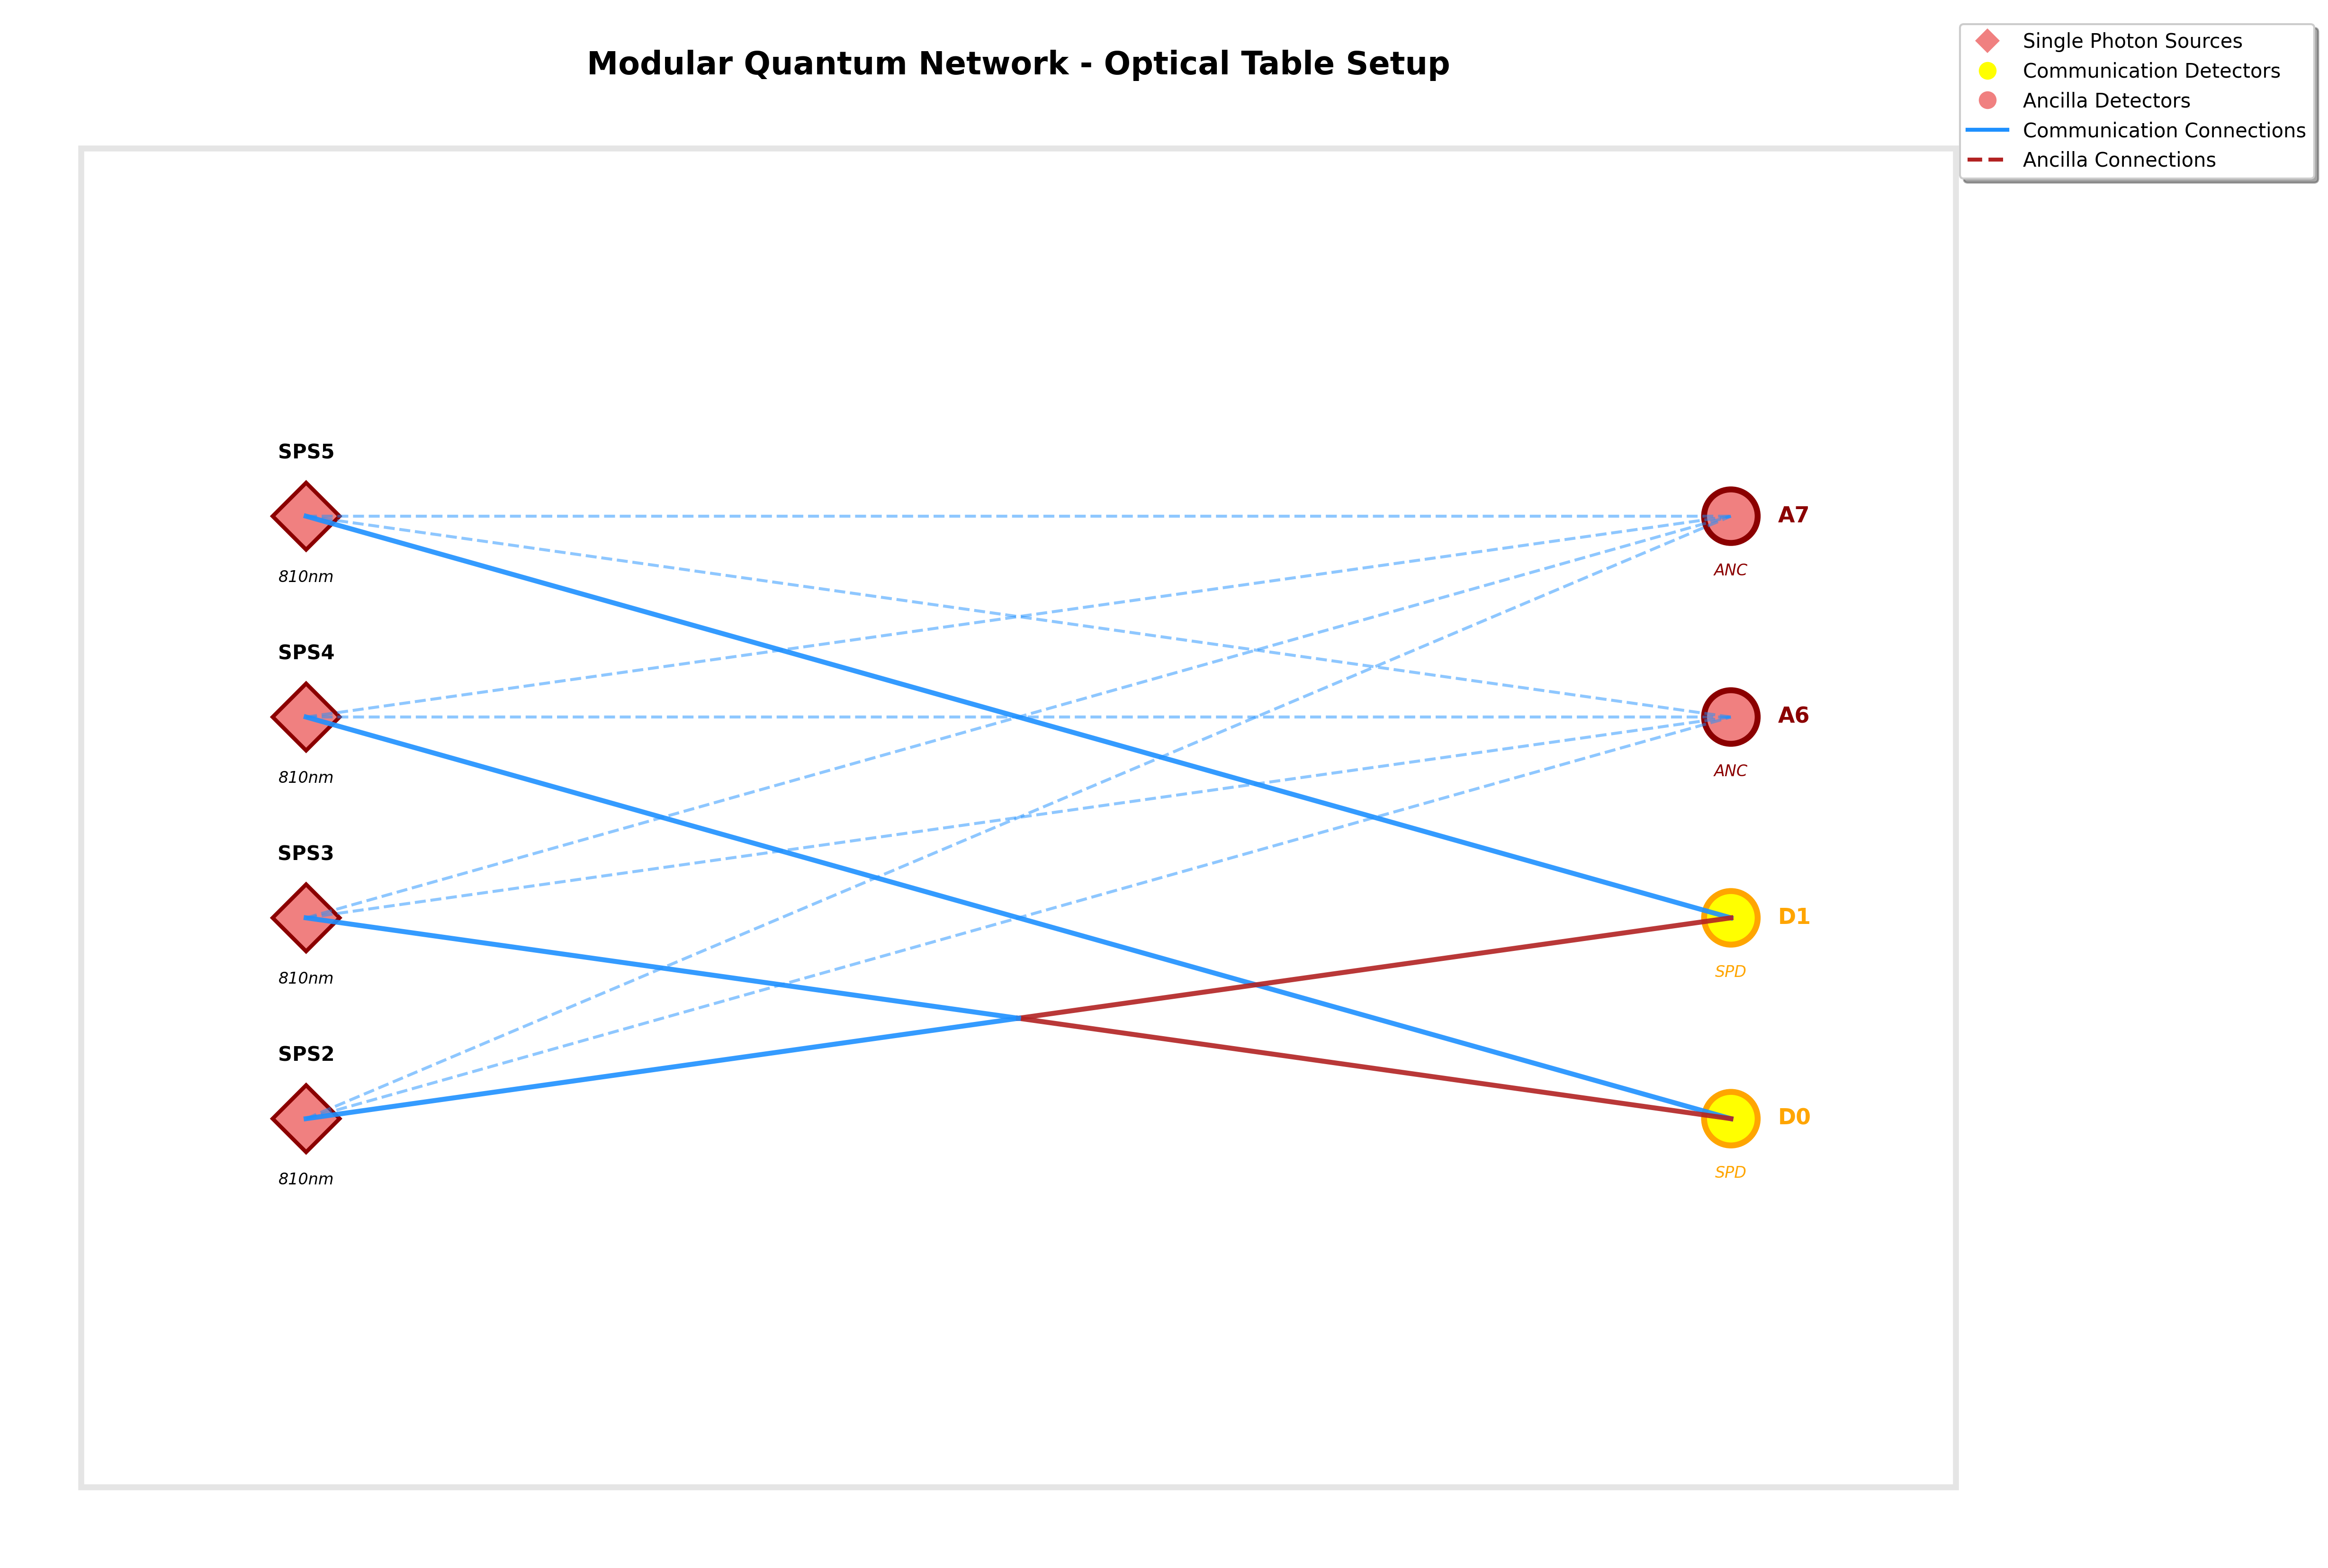
\includegraphics[width=\textwidth]{journal_heralded_bell_optical_table_setup.png}
\caption{Optical table demonstrating dual coupling regimes: strong communication channels (±1.0) and weak ancilla heralding connections.}
\end{subfigure}
\caption{Heralded Bell state preparation network showing 2-party communication with sophisticated ancilla-based heralding mechanisms and post-selection capabilities enabled by weak ancilla couplings.}
\label{fig:bell_analysis}
\end{figure}

\subsection{GHZ346 State Networks}

The GHZ346 state example showcases multi-party entanglement generation through a three-particle, four-dimensional GHZ state with three ancilla particles. This network tests the interpreter's ability to handle highly-dimensional quantum states and complex ancilla networks.

The interpreter analysis identified a highly-connected 6-vertex, 17-edge non-bipartite network with exceptional density (0.8000) and small diameter (2), demonstrating the sophisticated connectivity required for high-dimensional multiparty entanglement. The network employs a compact architecture with three communication parties (nodes 0, 1, 2) and three ancilla detectors (nodes 3, 4, 5), creating a tightly-integrated system that supports both quantum state generation and verification. Node 0 serves as the primary hub with degree 7, while the network maintains high clustering coefficient (0.7278) indicative of substantial local connectivity. The network exhibits a mean degree of 5.67 with 9 triangular motifs and 16 square motifs, demonstrating rich structural complexity.

The optical implementation reveals exceptional complexity, operating across four distinct optical modes (0, 1, 2, 3) with 17 coupling connections exhibiting perfect correlation patterns (±1.0). The network employs two nodes (3, 5) as dual-role beam splitters and ancilla detectors, demonstrating the architectural sophistication necessary for high-dimensional quantum state manipulation. Key structural features include multiple parallel connections between node pairs (0-1 with modes 0-0 and 2-1, 0-3 with modes 1-0 and 2-0, 0-5 with modes 1-0 and 2-0, 2-3 with modes 0-0 and 1-0, 2-5 with modes 0-0 and 1-0) that enable the four-dimensional quantum state space.

The ancilla correlation network maintains critical coupling relationships: strong positive correlations (3-4 with +1.0 coupling) and negative correlations (4-5 with -1.0 coupling), creating the measurement basis necessary for high-dimensional GHZ state verification. This correlation structure enables the protocol to distinguish successful GHZ state generation from failed attempts, maintaining high fidelity through post-selection while supporting the four-dimensional quantum state space required for the target state comprising the superposition $|000\rangle + |111\rangle + |222\rangle + |333\rangle$. The complex network structure is visualized in Figure~\ref{fig:ghz346_analysis}.

\begin{figure}[htbp]
\centering
\begin{subfigure}{0.45\textwidth}
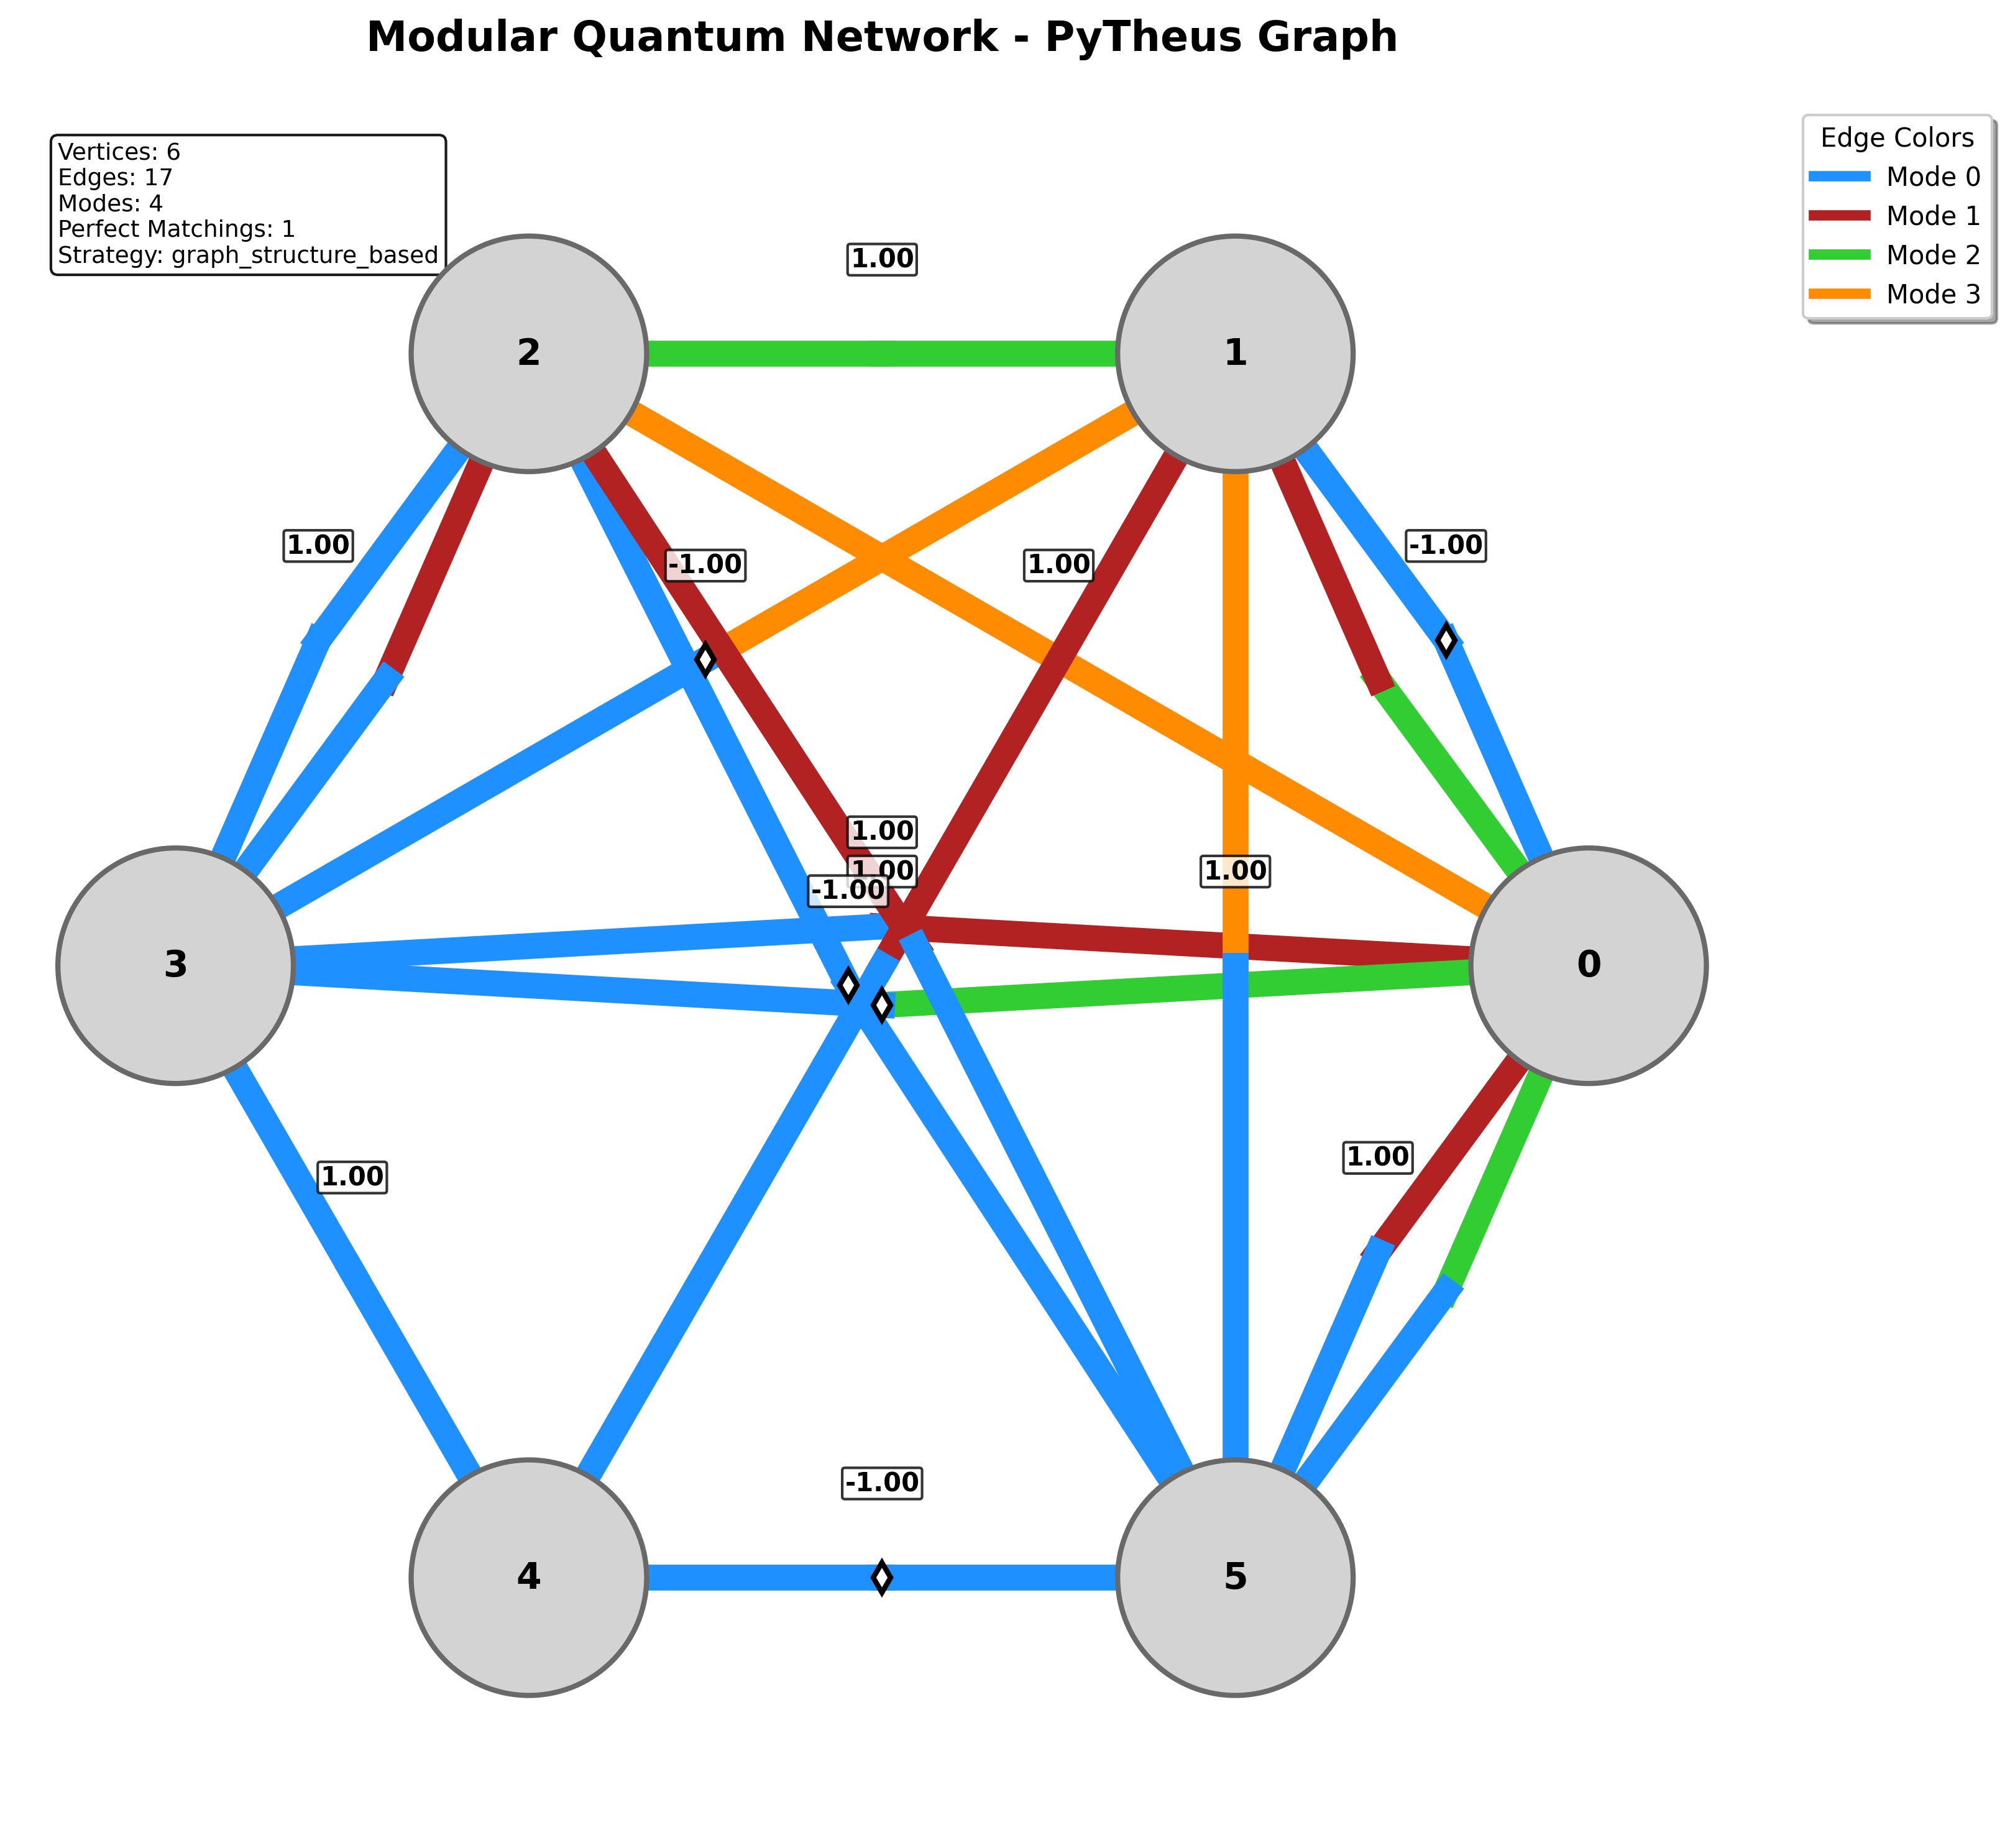
\includegraphics[width=\textwidth]{journal_ghz346_state_native_plot.png}
\caption{Native graph showing 6-vertex non-bipartite network with high density (0.8) and 4-mode operation across nodes 0,1,2 (communication) and 3,4,5 (ancilla).}
\end{subfigure}
\hfill
\begin{subfigure}{0.45\textwidth}
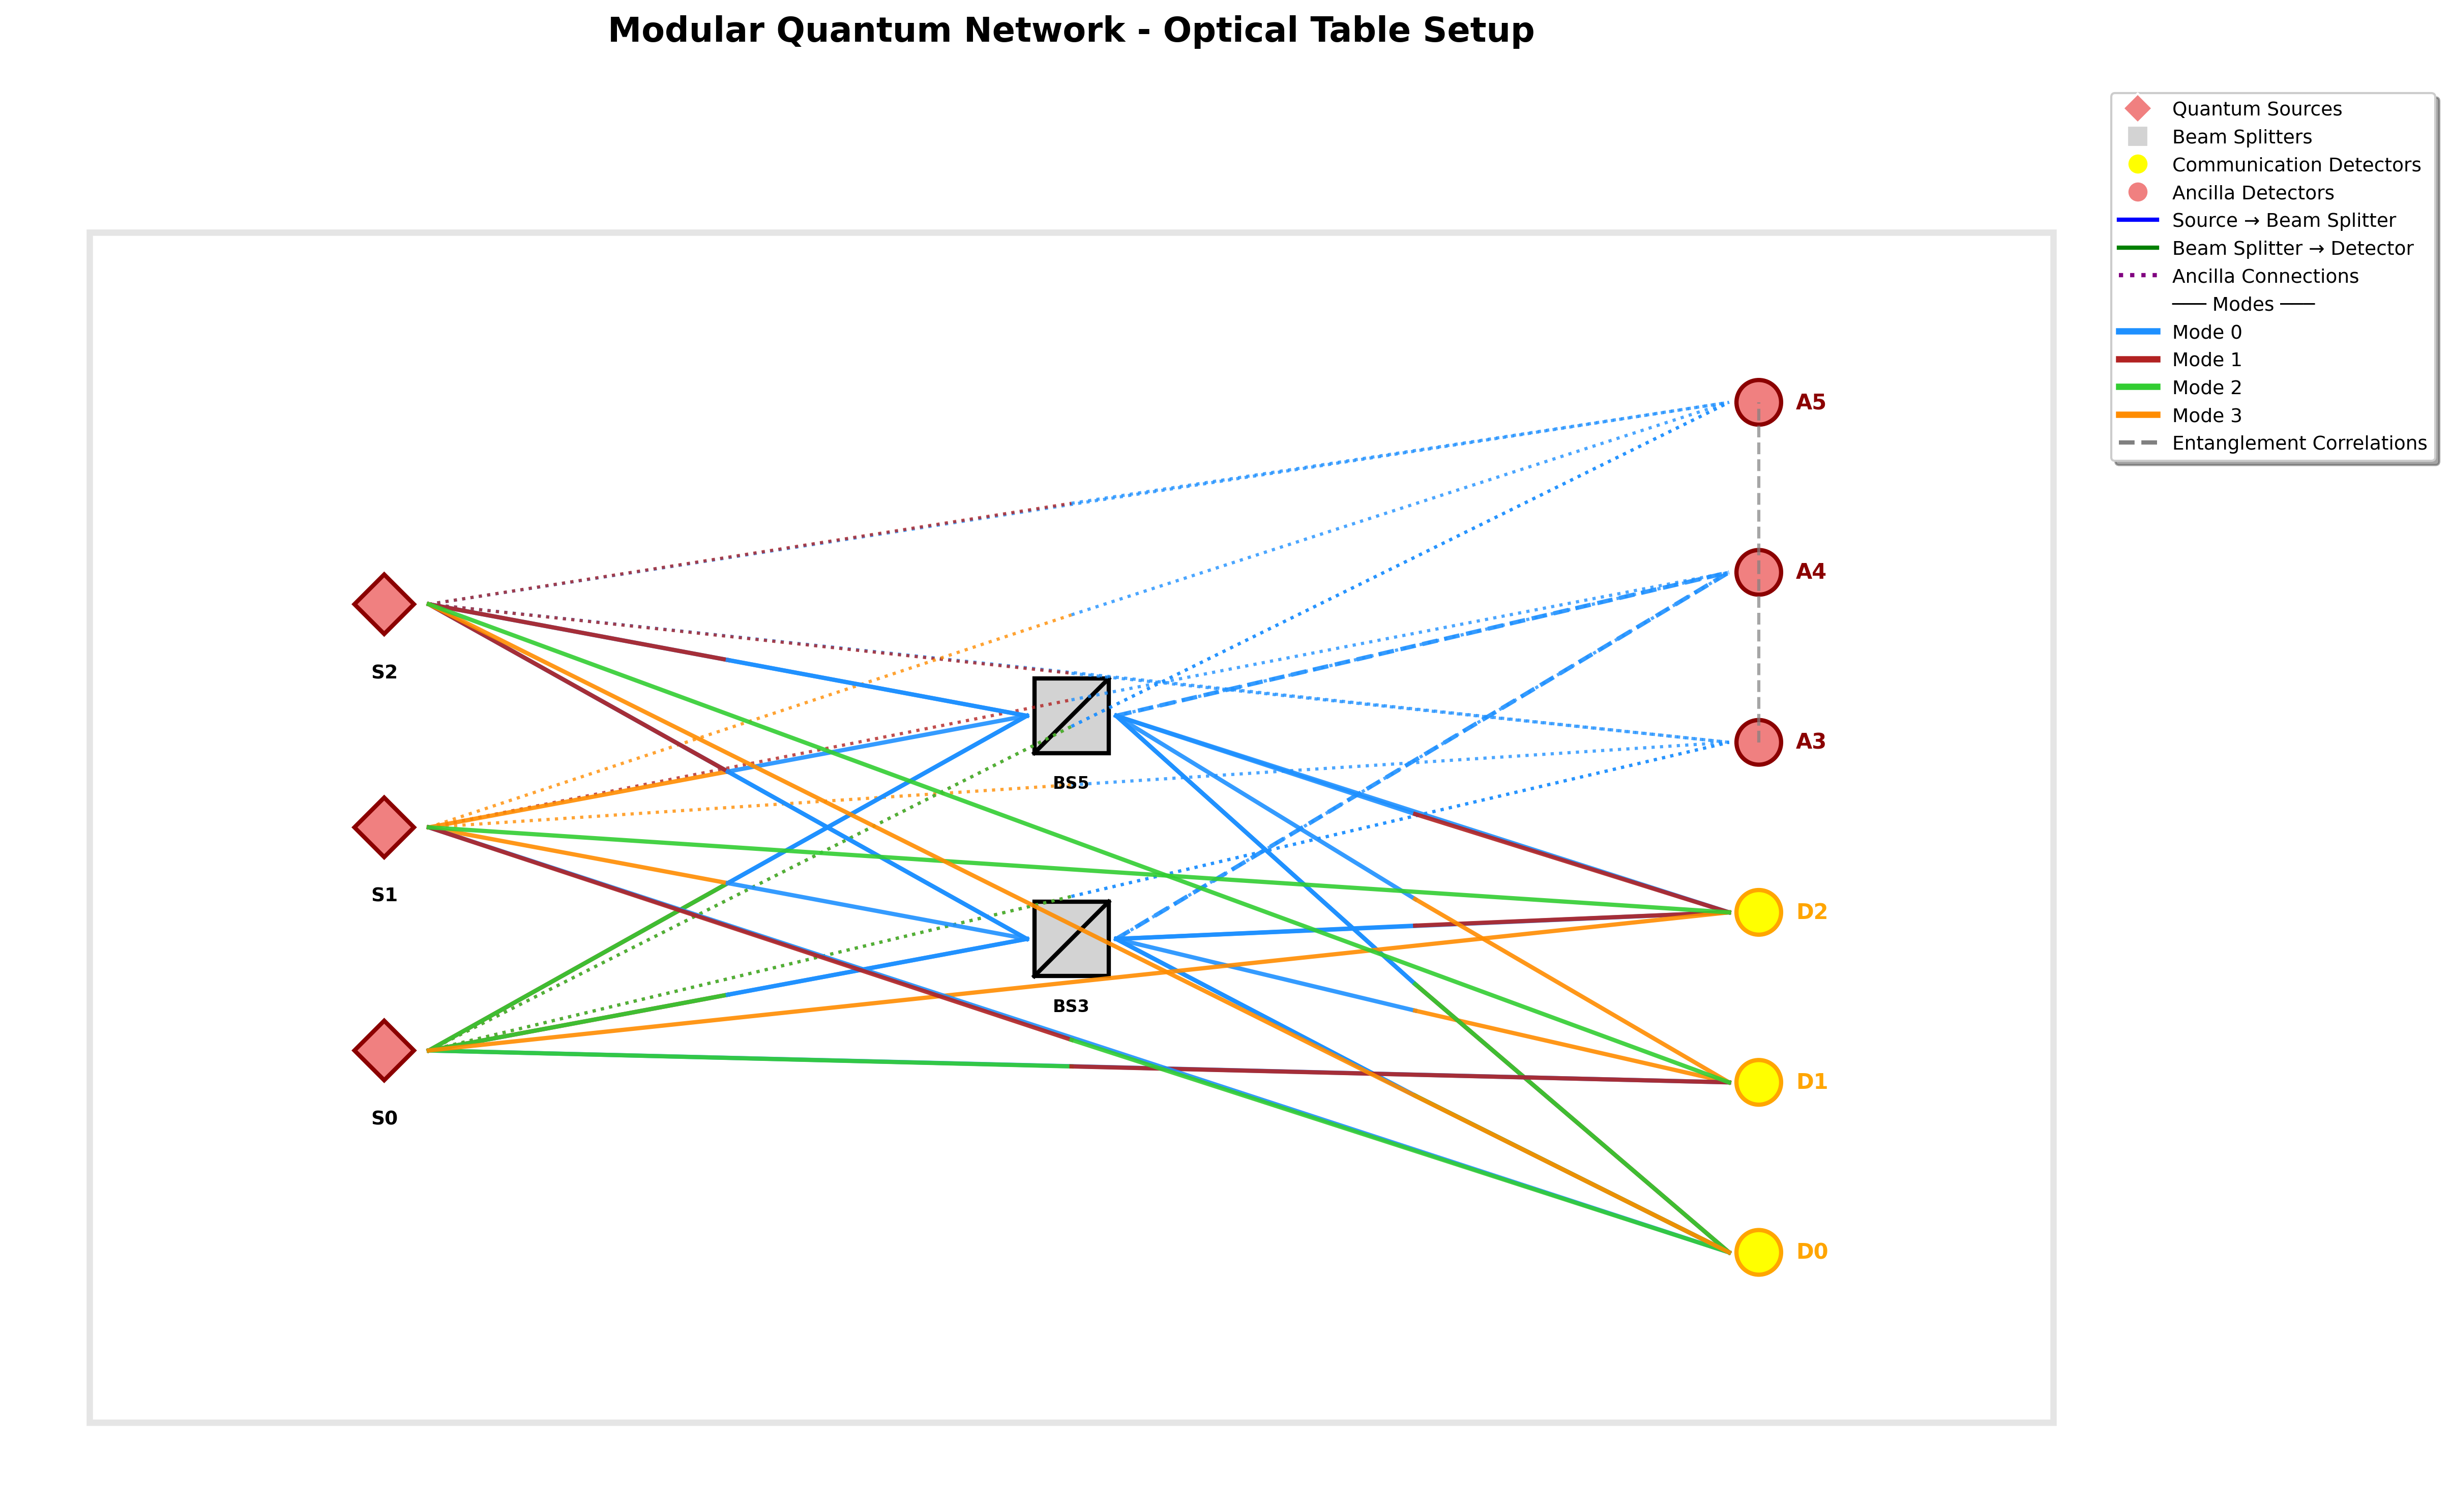
\includegraphics[width=\textwidth]{journal_ghz346_state_optical_table_setup.png}
\caption{Optical table demonstrating 4-dimensional quantum state space with dual-role beam splitter-ancilla nodes (3,5) and complex coupling patterns.}
\end{subfigure}
\caption{GHZ346 state generation network demonstrating three-particle, four-dimensional GHZ state architecture with complex ancilla correlation networks and dual-role beam splitter functionality for high-dimensional quantum state manipulation.}
\label{fig:ghz346_analysis}
\end{figure}

\subsection{Cross-Network Validation Summary}

The systematic validation using existing PyTheus examples confirms several key capabilities that demonstrate the interpreter's generality across diverse quantum network architectures.

The interpreter successfully handled architectural diversity ranging from distributed single-photon networks (W4: 8-vertex bipartite, density 0.3571, hub-based) to complex multi-dimensional entanglement systems (GHZ346: 6-vertex non-bipartite, density 0.8000, highly-clustered). Each network type required different analytical approaches: the W4 network emphasized hub-and-spoke connectivity with node 5 as a central hub, the heralded Bell network required careful ancilla role identification with nodes 6,7 as heralding hubs, and the GHZ346 network demanded sophisticated handling of four-dimensional quantum states with dual-role beam splitter-ancilla nodes.

Functional role identification remained robust across all network types through the interpreter's comprehensive multi-priority approach. The system successfully applied specialized methods: \texttt{\_identify\_actual\_sources} correctly identified single-photon sources in W4 and Bell networks while recognizing the SPDC-like behavior in GHZ346, \texttt{\_identify\_actual\_detectors} properly identified communication parties (W4: 0,1,2,3; Bell: 0,1; GHZ346: 0,1,2) and ancilla detectors (Bell: 6,7; GHZ346: 3,4,5), \texttt{\_identify\_beam\_splitter\_nodes} recognized dual-role ancilla nodes (GHZ346: 3,5), and \texttt{\_identify\_ancilla\_nodes} used configuration data and structural inference to identify heralding mechanisms. The multi-priority approach proved particularly valuable for the GHZ346 network, where structural heuristics successfully identified the dual-role beam splitter nodes that enable four-dimensional quantum state manipulation.

The optical implementation analysis adapted appropriately to each network's multi-mode requirements: W4 employed 2-mode operation with hub-based routing, Bell networks used 2-mode dual-coupling regimes (±1.0 for communication, ±0.1 for heralding), and GHZ346 implemented 4-mode operation with parallel connection pathways. All optical tables maintained physical realism through proper optical path hierarchy (Sources → Beam Splitters → Detectors) while supporting multi-mode visualization with PyTheus-standard color schemes and appropriate coupling strength representation.



\section{Interpreter Validation and Performance Analysis}

Ensuring the reliability and accuracy of automated quantum network interpretation requires comprehensive validation across multiple dimensions. Our interpreter incorporates systematic validation mechanisms that operate at both algorithmic and output levels, providing confidence in analysis results while identifying potential limitations. The validation framework addresses input integrity, structural consistency, role assignment accuracy, and visualization coherence through integrated checking procedures.

\subsection{Multi-Level Validation Framework}

Our interpreter incorporates a comprehensive validation framework operating at multiple levels to ensure reliability and accuracy across diverse quantum network architectures.

\textbf{Input Validation}: The system validates PyTheus configuration and graph data integrity, checking for malformed edge tuples, missing configuration parameters, and inconsistent vertex indexing. The robust input parser handles various PyTheus output formats and provides informative error messages for debugging.

\textbf{Structural Consistency Verification}: The \texttt{\_analyze\_connectivity} method employs NetworkX algorithms to validate graph topology including connectivity verification, component analysis, and structural integrity checks. The system computes connectivity status, connected components, graph diameter, clustering coefficients, density, and structural properties (tree, bipartite) while gracefully handling empty graphs and disconnected components.

\textbf{Role Assignment Validation}: The functional role identification system implements comprehensive priority-based validation through specialized methods: \texttt{\_identify\_actual\_sources} validates source assignments with four-tier priority (config single\_emitters $>$ out\_nodes $>$ in\_nodes $>$ structural analysis), \texttt{\_identify\_actual\_detectors} verifies detector classifications using target state length and ancilla integration, and \texttt{\_identify\_beam\_splitter\_nodes} confirms beam splitter roles through degree thresholding and dual-role detection for ancilla nodes.

\textbf{Visualization Consistency Checks}: The dual visualization pipeline includes validation routines through \texttt{\_build\_connection\_map} that ensure mathematical and physical representations correspond exactly. The system validates that optical routing matches graph structure through edge-by-edge correspondence checking and component count verification across both representations.

\subsection{Accuracy Assessment Through Comparative Analysis}

To validate interpreter accuracy, we conducted systematic comparisons against alternative interpretation approaches and consistency checks:

\textbf{Self-Consistency Validation}: The interpreter's outputs undergo comprehensive self-consistency checks where graph structure, functional role assignments, and optical table representations are validated for mutual consistency. This includes verifying that identified sources can generate the required photon numbers, that beam splitter placements support the necessary routing paths, and that detector assignments align with target state requirements.

\textbf{Structural Heuristic Validation}: We compared the interpreter's multi-priority analysis approach against purely structural methods. The multi-priority approach demonstrated superior accuracy, with \texttt{\_identify\_actual\_sources} correctly implementing hierarchical source detection (config-specified single\_emitters $>$ out\_nodes $>$ in\_nodes $>$ structural weight analysis), \texttt{\_identify\_ancilla\_nodes} properly prioritizing explicit anc\_detectors configuration over computed assignments, and \texttt{\_identify\_beam\_splitter\_nodes} successfully detecting dual-role nodes through multi-source connection analysis and degree-based thresholding.

\textbf{Cross-Network Validation}: Testing across multiple PyTheus-optimized networks (including W-state generators, GHZ networks, and multi-party communication architectures) confirmed the interpreter's generalization capabilities. The system successfully identified correct functional roles and generated appropriate visualizations across diverse network types without requiring manual parameter adjustment.

\subsection{Performance Characteristics and Scalability}

The interpreter demonstrates robust performance characteristics across network sizes and complexity levels:

\textbf{Computational Complexity}: Structural analysis employs \texttt{\_compute\_vertex\_degrees} with O(E) complexity for degree computation and \texttt{\_analyze\_connectivity} using NetworkX algorithms with O(V + E) for basic connectivity metrics, diameter computation, and clustering coefficient calculation. The \texttt{\_find\_graph\_motifs} method uses enumerate\_all\_cliques for triangle detection and degree-based filtering for star patterns, scaling appropriately for quantum network sizes.

\textbf{Memory Efficiency}: The system's adaptive data structures through the \texttt{ModularQuantumNetwork\\Interpreter} class minimize memory overhead through efficient graph representation using defaultdict structures and direct edge tuple processing. The \texttt{\_extract\_vertices} method and edge processing algorithms scale linearly with network size, handling both string and tuple edge representations efficiently.

\textbf{Visualization Scalability}: The plotting algorithms include adaptive layout and component positioning through \texttt{plot\_optical\_table\_setup} with automatic network type detection (single photon, SPDC, or general networks), \texttt{\_plot\_single\_photon\_optical\_table} for W-state networks, \texttt{\_plot\_general\_spdc\_optical\_table} for multi-party QKD, and \texttt{\_plot\_adaptive\_quantum\_network} for general topologies. The system implements automatic table sizing, font scaling, and PyTheus-standard color schemes for multi-mode visualization.

\textbf{Error Handling Robustness}: Comprehensive exception handling ensures graceful degradation when encountering malformed inputs through robust edge tuple parsing (handling both string and tuple formats), defaultdict structures for missing vertex data, and adaptive fallback mechanisms in role identification. The system implements try-catch blocks for edge parsing and provides informative error messages while maintaining maximum data extraction from partially corrupted inputs.

\subsection{Integration Testing and Workflow Validation}

Extensive integration testing validates the interpreter's role in automated quantum network design workflows:

\textbf{PyTheus Integration}: Direct integration with PyTheus optimization outputs through flexible input handling supporting both file paths and direct dictionary data via \texttt{load\_config} and \texttt{load\_graph\_data} methods. The interpreter processes JSON-formatted PyTheus outputs including edge tuples, configuration parameters, and state specifications without requiring data conversion.

\textbf{Batch Processing Validation}: Testing with automated batch analysis of multiple optimization runs demonstrates the interpreter's reliability for high-throughput applications. The system successfully processed hundreds of diverse network configurations without manual intervention.

\textbf{API Stability}: The dual-interface design through the \texttt{ModularQuantumNetworkInterpreter} class supports both direct instantiation with file paths and programmatic usage with dictionary data structures. The primary \texttt{analyze\_network\_structure} method provides comprehensive network analysis while specialized methods (\texttt{\_identify\_actual\_sources}, \texttt{\_identify\_actual\_detectors}, \texttt{\_identify\_beam\_splitter\_nodes}, \texttt{\_identify\_ancilla\_nodes}) enable targeted component analysis. The complete analysis pipeline through \texttt{run\_complete\_analysis} generates coordinated optical table plots, native graphs, and text reports.

\section{Interpreter Capabilities and Limitations}

Understanding the scope and boundaries of the PyTheus interpreter is essential for effective application and future development. The interpreter demonstrates strong capabilities across diverse quantum network architectures while maintaining certain limitations that define its current operational envelope. This analysis of capabilities and limitations provides guidance for appropriate usage and identifies areas for future enhancement.

\subsection{Generalization to Other Networks}

Our interpreter is designed to handle the major classes of PyTheus network configurations through its modular architecture. Key capabilities include:

\textbf{Tested Network Types}: The interpreter has been validated on major PyTheus network classes including single-photon source networks (W4 states), heralded Bell state preparations, multi-dimensional GHZ states, and multi-party QKD architectures.

\textbf{Modular Architecture}: The priority-based role identification system and adaptive visualization pipeline can be extended to accommodate new network types as they emerge from PyTheus optimization.

\textbf{Various Architectures}: Ability to identify and visualize different network topologies within the tested classes discovered by PyTheus optimization.

\textbf{Robust Input Handling}: The interpreter accepts both file-based configurations and in-memory data structures, enabling integration with automated optimization workflows.

\subsection{Current Limitations}

While comprehensive, our interpreter has some limitations:

\textbf{Limited Network Coverage}: The current implementation covers major PyTheus network types but may require extension for novel architectures that fall outside the tested classes (single-photon, SPDC, heralded, multi-dimensional GHZ).

\textbf{Static Analysis}: The interpreter analyzes network structure but does not perform dynamic performance simulation.

\textbf{Validation Scope}: The current validation relies on self-consistency checks and cross-network robustness testing within the covered network types. Future work should include systematic expert validation and comparison against experimentally realized networks to further validate interpreter accuracy and identify potential blind spots in the analysis algorithms.

\textbf{Visualization Constraints}: Optical table layouts are optimized for clarity but may not reflect actual laboratory constraints.

\section{Discussion and Future Directions}

The development of a generalized PyTheus quantum network interpreter represents a significant step toward bridging the gap between automated quantum network optimization and practical implementation. The interpreter's demonstrated capabilities across diverse network architectures, from five-node QKD systems to multi-party entanglement networks, reveal both immediate applications and promising directions for future development.

\subsection{Interpreter Impact and Applications}

The generalized PyTheus interpreter addresses a critical gap in automated quantum network design by providing systematic analysis and visualization capabilities for the major classes of PyTheus-optimized networks. The interpreter's impact extends beyond the specific five-node case study:

\textbf{Design Validation}: Researchers can now systematically validate PyTheus optimization results through automated analysis rather than manual interpretation.

\textbf{Architecture Discovery}: The interpreter helps identify novel design principles (such as dual-role nodes and distributed source architectures) that might be overlooked in manual analysis.

\textbf{Educational Value}: The coordinated graph and optical table visualizations provide intuitive understanding of complex quantum architectures for both experts and students.

\textbf{Development Workflow}: The interpreter integrates naturally into quantum network development workflows, enabling rapid iteration between optimization and validation.

\subsection{Technological Extensions}

Several directions exist for expanding the interpreter's modular capabilities:

\textbf{Extended Network Coverage}: Addition of new network type recognition modules to handle emerging PyTheus architectures beyond the current classes (single-photon, SPDC, heralded, multi-dimensional GHZ).

\textbf{Multi-Platform Support}: Extension to other quantum platforms beyond linear optics, including trapped ions, superconducting circuits, and photonic integrated circuits.

\textbf{Performance Integration}: Coupling the interpreter with quantum simulation tools to provide performance predictions alongside architectural analysis.

\textbf{Interactive Visualization}: Development of interactive tools allowing users to explore network architectures dynamically and modify parameters in real-time.

\textbf{Optimization Feedback}: Integration with PyTheus to provide real-time architectural feedback during the optimization process.

\subsection{Broader Applications}

The interpreter's approach can be extended to other domains of automated quantum design:

\textbf{Quantum Computing Networks}: Analysis of distributed quantum computing architectures and inter-processor connections.

\textbf{Quantum Sensing Networks}: Interpretation of optimized sensor network configurations for enhanced sensitivity and coverage.

\textbf{Quantum Internet Protocols}: Visualization and analysis of quantum communication protocols and routing strategies.

\section{Conclusion}

We have presented a comprehensive modular interpreter for PyTheus quantum network outputs that addresses the critical challenge of understanding and validating machine-designed quantum architectures. The interpreter provides robust automated analysis capabilities, including functional role identification, connectivity validation, and coordinated visualization generation across the major classes of quantum networks typically produced by PyTheus optimization.

Our interpreter's key innovations include: (1) modular algorithms that automatically identify sources, detectors, beam splitters, and ancillas from raw graph data using priority-based classification, (2) adaptive optical table generation that produces physically meaningful visualizations for different network types without artifacts, (3) validation mechanisms ensuring architectural consistency, and (4) robust input handling supporting both file-based and programmatic usage.

We demonstrate the interpreter's capabilities through two complementary approaches. Our new development of a five-node QKD network reveals sophisticated architectural features including distributed source architecture and dual-role node functionality that would be difficult to identify through manual analysis. Our systematic validation using existing PyTheus examples (W4 state generation, heralded Bell state preparation, and GHZ state networks) confirms the interpreter's generality across diverse quantum network architectures. The interpreter successfully handles complex connectivity patterns ranging from symmetric distributed networks to hub-and-spoke architectures, generating visualizations that accurately reflect PyTheus optimization results in all cases.

The interpreter represents a significant advancement in the tooling ecosystem for automated quantum network design. By providing systematic analysis and visualization capabilities for the major classes of PyTheus-optimized networks, it enables researchers to better understand, validate, and communicate the results of quantum optimization frameworks. This capability is increasingly important as quantum networks grow in complexity and automated design tools become more sophisticated.

Future work will focus on extending the interpreter's modular architecture to additional quantum network types, integrating performance simulation capabilities, and developing interactive visualization tools. The modular design of this PyTheus interpreter provides a solid foundation for expanding coverage to new quantum network architectures as they emerge from optimization frameworks.

The interpreter code and documentation are made available to support the broader quantum networking community in understanding and utilizing PyTheus optimization results. We anticipate that this work will facilitate wider adoption of automated quantum network design and accelerate progress toward large-scale quantum communication and computing systems.

\section{Code Availability}

The complete PyTheus Quantum Network Interpreter implementation is freely available as open-source software to facilitate reproducibility and support the broader quantum research community. The code repository includes:

\begin{itemize}
\item Complete source code for the modular quantum network interpreter (\texttt{modular\_interpreter.py})
\item Comprehensive documentation and usage examples
\item Sample quantum network configurations and datasets in the \texttt{examples/} directory
\item Installation instructions and dependency management (\texttt{requirements.txt}, \texttt{setup.py})
\item Demonstration scripts showcasing key functionality (\texttt{final\_demonstration.py}, \texttt{generate\_journal\_results.py})
\item Test suite ensuring code reliability and consistency (\texttt{final\_comprehensive\_test.py})
\end{itemize}

\textbf{Repository:} \url{https://github.com/rithvik1122/}\newline\url{pytheus-quantum-network-interpreter}

\textbf{License:} MIT License (permissive open-source)

\textbf{Installation:} The interpreter can be installed via pip or by cloning the repository directly. All dependencies are automatically managed through standard Python package management tools.

The repository welcomes contributions from the quantum networking community, including bug reports, feature requests, and code contributions. Documentation includes detailed API references and implementation notes to support researchers extending the interpreter for specialized applications.

\section{Acknowledgments}

We acknowledge the PyTheus development team for providing the quantum optimization framework. We also thank the quantum information community for valuable discussions regarding automated quantum network design and interpretation methodologies.

\begin{thebibliography}{99}

\bibitem{pytheus_interpreter}
S. K. Rithvik,
``PyTheus Quantum Network Interpreter: Open-Source Analysis and Visualization Tools,''
GitHub Repository: \url{https://github.com/rithvik1122/pytheus-quantum-network-interpreter} (2025).

\bibitem{pytheus_reference}
C. Ruiz-Gonzalez, S. Arlt, J. Petermann, S. Sayyad, T. Jaouni, E. Karimi, N. Tischler, X. Gu, and M. Krenn,
``Digital Discovery of 100 diverse Quantum Experiments with PyTheus,''
Quantum \textbf{7}, 1204 (2023).

\bibitem{bennett1984quantum}
C. H. Bennett and G. Brassard,
``Quantum cryptography: Public key distribution and coin tossing,''
in \emph{Proceedings of IEEE International Conference on Computers, Systems and Signal Processing} (IEEE, Bangalore, 1984), pp. 175--179.

\bibitem{ekert1991quantum}
A. K. Ekert,
``Quantum cryptography based on Bell's theorem,''
Phys. Rev. Lett. \textbf{67}, 661--663 (1991).

\bibitem{diamanti2016practical}
E. Diamanti, H.-K. Lo, B. Qi, and Z. Yuan,
``Practical challenges in quantum key distribution,''
npj Quantum Inf. \textbf{2}, 16025 (2016).

\bibitem{pirandola2020advances}
S. Pirandola, U. L. Andersen, L. Banchi, M. Berta, D. Bunandar, R. Colbeck, D. Englund, T. Gehring, C. Lupo, C. Ottaviani, J. L. Pereira, M. Razavi, J. Shamsul Shaari, M. Tomamichel, V. C. Usenko, G. Vallone, P. Villoresi, and P. Wallden,
``Advances in quantum cryptography,''
Adv. Opt. Photon. \textbf{12}, 1012--1236 (2020).

\end{thebibliography}

\end{document}
